% This file should be replaced with your file with an thesis content.
%=========================================================================
% Authors: Michal Bidlo, Bohuslav Křena, Jaroslav Dytrych, Petr Veigend and Adam Herout 2019

% For compilation piecewise (see projekt.tex), it is necessary to uncomment it and change
% \documentclass[../projekt.tex]{subfiles}
% \begin{document}

\chapter{Introduction}

The concept of finite state automaton was first introduced by two neurophysiologists, Warren McCulloch and Walter Pitts, in 1943 \cite{Wolfram2002}. Later, this concept was further developed by computer scientists G.H. Mealy and E.F. Moore, who created a model of a machine transitioning over a set of states while producing output based on its given input. This can be considered the base for the finite state automata (FSAs) we know today \cite{Standford2004}.

Since then, FSAs have found their usage in a wide range of applications like speech recognition, text parsing, static verification and validation, or protocol analyses. Essentially everything that can be defined as a series of states can be represented by an FSA. In static verification and validation, finite state automata are used to represent a state space of a given program, in lexical analyzers, they are used to check whether given sets of characters match the required pattern and are valid to proceed further. Finite state automata can also be found in everyday appliances without us even noticing, such as vending machines or elevators, whose actions are determined by the input they are given, and the state they are currently in~\cite{Wright2005}.


While there is no doubt that FSAs are a useful structure in information technology, working with them can be found impractical when their size reaches a certain limit. The main advantage of FSAs is the small memory they need to operate. As their actions are based only on the state they are in and the input that is given, these are the only parameters that need to be stored. However, that cannot be said about the data structure storing the automaton itself. In real-life applications, some automata can explode in size and consist of an enormous number of states and transitions.
Working with such vast data structures is found inefficient, and that is where the idea of automata reduction found its place.


Since multiple FSA can describe the same language, it is logical that we want to operate with the smallest one possible. Since we start with our original potentially inefficient automaton, we are looking for an algorithm that transforms that automaton into another with the same language but a smaller number of states and transitions. Even though this kind of operation on a large automaton can be costly in the processing time needed for it to be done, usually the reduction is wanted, especially in cases when the automaton is used multiple times.
Generally, we can speak about two different types of automata reductions, which are the reduction of deterministic automata and the reduction of nondeterministic automata.


Deterministic automata (DFAs) are restricted to a single transition for each symbol for a state. Because of this deterministic property, which does not allow any ambiguities, DFAs are limited in their complexity. This can cause their size to be exponential compared to the size of a nondeterministic automaton representing the same language. On the other hand, their simpler concept makes them more suitable for methodical and algorithmic work. The reduction of deterministic automata is often considered a closed topic because of the possibility of finding the minimal deterministic automaton through multiple algorithms. In our thesis, we will be looking at Hopcroft's and Brzozowski's algorithms. In the worst-case scenario, they run in loglinear and exponential time, respectively, and they are always guaranteed to find the smallest deterministic equivalent to the given automaton. With such good enough results, those reductions are still widely used even these days. In our work, they set the standard to which the other types of reduction will be compared.


The same algorithms cannot be applied to nondeterministic automata without determinizing them first. Nondeterministic automata (NFAs) are not limited by the deterministic property as the DFAs are, which grants them the ability to define languages more compactly. Determinization would cause expansion of the automaton, which could mean that even after reduction, the final automaton would still be bigger than the original nondeterministic one. To utilize the NFAs' ability to the fullest, it would be beneficial to reduce automata directly from their nondeterministic version. Finding the smallest NFA with equivalent language is proven to be a PSPACE-complete problem, which makes NFA reduction computationally hard~\cite{Jiang93}. For this reason, it is still considered an intriguing topic when different types of reduction have each their strengths. We looked at two nondeterministic reductions, in particular, the reduction using the relation of simulation and the reduction through the residual automata.

The article \textit{Liveness of Randomised Parameterised Systems under Arbitrary Schedulers}~\cite{Lin2016} presented a new way of looking at FSAs. The main idea of their work was to prove the liveness of randomized parameterized systems exploiting boolean satisfiability problem (SAT) solvers. They created a formula for representing such a problem as a clause in conjunctive normal form (CNF), which is then solvable using the solver. Inspired by this idea, we tried to implement it for our problem of automata reduction. We represented the structure of an FSA as a clause in the CNF defining its language by two sets of example words, which the automaton accepts and rejects, respectively. This process may seem inefficient since there is an excessive number of words in a single automaton language, and it is impossible to predict how many example words will be required to find a language-equivalent automaton. As this means that the clause defining the automaton could be massive, the results of this algorithm could be highly dependent on the used solver as well as the exact automaton and the example words used. For this reason, we focused on smaller-sized automata to prove the possibility of finding minimal equivalent FSA using SAT solvers.

We expanded this idea also onto nondeterministic automata using quantified boolean formula (QBF) solvers, where we can utilize the quantified variables to efficiently represent the multiple paths leading from a single state.

In Chapter \ref{chap:theory} is defined the theoretical background for this thesis. Chapter \ref{chap:reduction} contains the descriptions of selected reduction algorithms that were implemented for this work. Our created method for denoting an FSA as a CNF formula and an algorithm utilizing SAT and QBF solvers for reduction is described in Chapter \ref{chap:sat_qbf}. Chapter \ref{chap:implementation} includes the finer details of the implementation together with used file formats and Chapter \ref{chap:evaluation} shows the results from experimental evaluation of each type of reduction implemented. Chapter \ref{chap:conclu} contains the overall summary of this thesis and possibilities for future work.


\chapter{Preliminaries and Definitions}
\label{chap:theory}

In this chapter, we will summarize the theoretical notion used in the thesis together with definitions. Firstly we will define the concept of nondeterministic finite state automata, their language, equivalence, and the meaning of reverse automata. Then we will set the definitions for deterministic automata together with complement automata and the explanation of the concept of determinization~\cite{Maheshwari2019, Sipser2006}. Lastly, we define the fundamentals of propositional logic, the problematics of SAT and QBF solvers, and methods of formula transformation into CNF~\cite{Abdulla2010, GaneshV20, Keef2023, Masina2023, Prince2020, Sipser2006, SAV}.

\section{Nondeterministic Finite State Automaton}
\label{sec:NFA}

A \textbf{nondeterministic finite state automaton} (NFA) is a type of FSA that we can formally define as a tuple $M_{NFA}=(Q, \Sigma, R, I, F)$ where:

\begin{itemize}
    \item $Q$ is a nonempty finite set of states,
    \item $\Sigma$ is a nonempty finite set of input symbols called an \textit{alphabet},
    \item $R$ is a transition function in a form of $Q\times (\Sigma \cup \{\varepsilon \})  \to P(Q)$, where $P(Q)$ is a collection of all subsets of $Q$,
    
    \begin{itemize}
        \item we denote a transition from state $p$ to state $q$ through symbol $a$ as $r_{paq}\colon p\xrightarrow{a}q$ where $q,p \in Q$ and $a \in \Sigma$, 
        \item we use notation $R(q,a)$ for all states reachable from state $q \in Q$ using a transition through symbol $a \in \Sigma$,
    \end{itemize}
    
    \item $I$ is a nonempty set of initial (or starting) states, $I \subseteq Q$, and
    \item $F$ is a set of accepting (or final) states, $F \subseteq Q$.
\end{itemize}

It is preferred to describe FSA visually through state diagrams, which makes them easier to comprehend and visualize (Figure \ref{NFA}). \\

\begin{figure}[ht]
    \label{NFA}
    \centering
    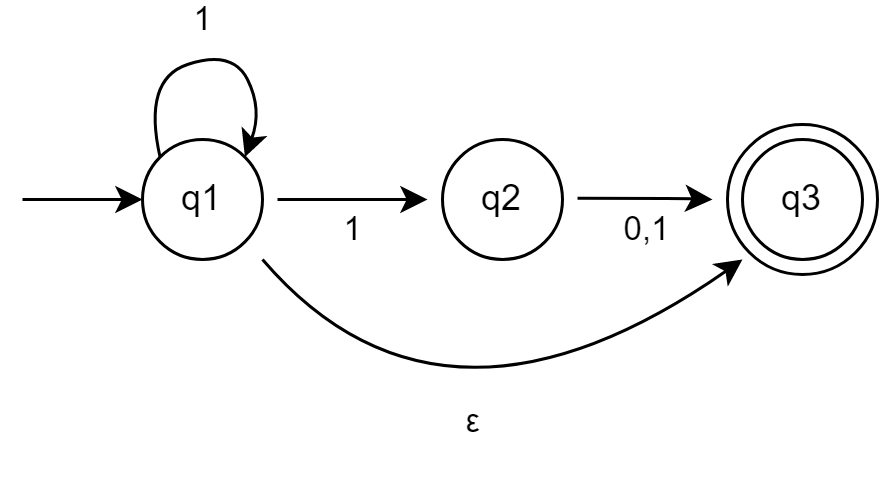
\includegraphics[width=0.5\linewidth]{obrazky-figures/NFA.drawio.png}
    \caption{State diagram of an NFA with three states $Q=\{q1, q2, q3\}$, an initial state $I=\{q1\}$, a final state $F=\{q3\}$, a binary alphabet $\Sigma = \{0, 1\}$, and transition function $R=\{q_1 \xrightarrow{1} q_1,q_1 \xrightarrow{1} q_2,q_1 \xrightarrow{\varepsilon} q_3, q_2 \xrightarrow{0} q_3, q_2 \xrightarrow{1} q_3\}$ represented by arrows with input symbols in the diagram.}
\end{figure}

\textbf{Epsilon transition} (marked with symbol $\varepsilon$) refers to a particular type of transition characteristic for NFAs. Such transitions are possible to be taken directly without requiring any input as can be seen in our example automaton (Figure \ref{NFA}) that is able to proceed from state $q1$ to $q3$ immediately.

The automata can have an infinite number of transitions over a finite word using these transitions as shown in Figure \ref{eps_cycle}. For this inconvenience, these transitions are often eliminated or never used in the first place. Their replacement can be observed in the process of determinization in Section \ref{ssec:num2.4}. Unless otherwise stated, we anticipate that these transitions will not be present in the automata for further definitions or algorithms. \\

 \begin{figure}[ht]
    \label{eps_cycle}
    \centering
    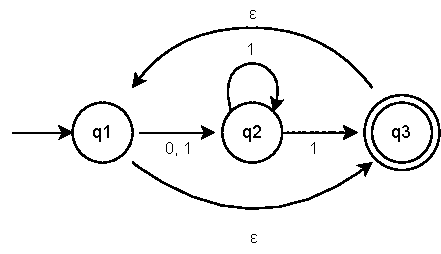
\includegraphics[width=0.5\linewidth]{obrazky-figures/epsilon_cycle.drawio.pdf}
    \caption{NFA automaton with epsilon transitions causing an infinite loop without taking any symbol as an input. As a result, for any input word, there exists an endless path.}
\end{figure}

The main attribute of an NFA is its ambiguity caused by the possibility of multiple transitions leading from a single state. That means that an input word is accepted if at least one of the numerous paths in the automaton ends in an accepting state. As a result of this ability, NFAs can define a language more compactly with fewer states, which makes them more likely to be used.


\subsection*{Language of a Finite State Automaton}
An~\textbf{alphabet} ${\Sigma=\{a_1, a_2, \dots, a_n\}}$ represents a~nonempty finite set of symbols that the automaton takes as its input as defined in the previous section. A~\textbf{word} ${a_1 a_2 \dots a_n \in \Sigma^*}$ is a sequence of such symbols.

A~\textbf{run} over an~input word ${a_1 a_2 \dots a_n}$ creates a~\textit{path} from an initial state, which can be defined as a series of transitions ${q_1 \xrightarrow{a_1} q_2 \xrightarrow{a_2} \dots \xrightarrow{a_n} q_{n+1}}$, ${q_1 \in I}, {q_1,q_2,...,q_{n+1} \in Q}$.
An automaton \textit{accepts a~word} ${a_1a_2...a_n}$ if there exists a path starting from an initial state and ending in an accepting state, formally written as ${q_1 \xrightarrow{a_1} q_2 \xrightarrow{a_2} \dots \xrightarrow{a_n} q_{n+1}}$, ${q_1 \in I}, {q_n \in F}$, $ {q_1,q_2,...,q_{n+1} \in Q}$.
Otherwise the \textit{word is rejected}.

\textbf{Automaton language} is a set of all words that an automaton accepts. \\

\textbf{Regular expressions} (regexes) are generally used to describe an~automaton language that follows the following set of rules:
\begin{itemize}
    \item regexes $\varepsilon$ and $\emptyset$ denote the languages \{$\varepsilon$\} and $\emptyset$ accordingly,
    \item for each $a \in \Sigma$ regex $a$ denotes the language $\{a\}$,
    \item regex $a+b$ denotes the language created by union of regexes $a$ and $b$,
    \item regex $ab$ denotes the language created by concatenation of regexes $a$ and $b$, and
    \item regex $a^*$ denotes the language of zero and more occurrences of the language of the regex a.
\end{itemize}
 For example, the automaton from Figure~\ref{NFA} represents the language equal to the regex ${1^*((10)+\varepsilon)}$ describing the language ${L=\{\varepsilon, 1, 10, 11, 110, 111, 1110, 1111, \dots \}}$. We can find two extreme cases of languages and that is the \textit{empty language} $L=\emptyset$, which is a language with no words. On the other side, we have the language $L={\Sigma^*}$ consisting of all possible words that could be created from the alphabet plus the empty string.

\subsection*{Reverse Finite State Automaton}
Let $M=(Q,\Sigma, R, I, F)$ be an NFA. The \textbf{reverse automaton} $M_R=(Q,\Sigma, R_R, I_R, F_R)$ to automaton $M$ is then defined as $I_R = F$, $F_R = I$ and $R_R$ is a reversed transition function to function $R$ meaning that:
\begin{equation*}
    R_R=\{p_1 \xrightarrow{a} p_2\mid\ p_2 \xrightarrow{a} p_1 \in R\}
\end{equation*} 
For an example of the reverse automaton see Figure \ref{fig:rev_auto}.

\begin{figure}[ht]
    \label{fig:rev_auto}
    \centering
    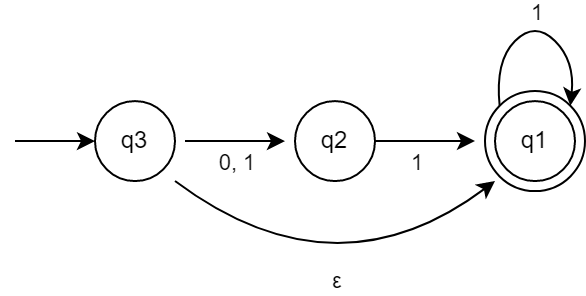
\includegraphics[width=0.5\linewidth]{obrazky-figures/reverse_auto.png}
    \caption{An~example of the reverse automaton constructed to the automaton from Figure \ref{NFA}.}
\end{figure}

\subsection*{Automata Equivalence}
Two automata $M_1, M_2$ are considered \textit{language-equivalent} if they define the same language $L_{M_1} = L_{M_2}$. Equivalence of languages $L_1, L_2$ can be defined as
\begin{equation*}
    L_1 = L_2 \iff (L_{M_1} \cap L_{C(M_{2})}) \cup (L_{M_2} \cap L_{C(M_{1})}) = \emptyset,
\end{equation*} where $C(M_{1}), C(M_{2})$ are complement automata to $M_1$ and $M_2$. For complement automata see the last part of Section \ref{sec:dfa}.

\textbf{Antichains} provide a different method of checking the equivalence of languages of the automata that does not require creating complements. Let ${M_{NFA}=(Q_M,\Sigma, R_M, I_M, F_M)}$ and ${N_{NFA}=(Q_N,\Sigma, R_N, I_N, F_N)}$ be two automata such that $Q_M \cap Q_N = \emptyset$. A \textbf{product automaton} is denoted by $M\times N$, where a state of this automaton is a pair $(p, P)$, where $p \in Q_M$ and $P \subseteq Q_N$ is a set of states of automaton $N$. It holds that $L_M \subseteq L_N$ if there is no such state $(p, P)$ in the product automaton of those automata that $p$ is an accepting state while $P$ is not, formally:
\begin{equation*}
    L_M \subseteq L_N \iff \nexists (p, P) \in M\times N: p \in F_M \land P \cap F_N = \emptyset
\end{equation*}
Generally, traversing the whole product automaton is needed to ensure that the language of automaton $M$ is a subset or equal to the language of automaton $N$. However, the antichains method introduces a condition that the search from state $(p, P)$ can be stopped if there exists a state $(p, R)$ that was already visited, and it holds that $R \subseteq P$. The equivalence of the automata's languages may therefore be verified more effectively with antichains.

\section{Deterministic Finite State Automaton}
\label{sec:dfa}
A \textbf{deterministic finite state automaton} (DFA) is a special type of NFA for which it holds that in every state of the automaton, it is precisely given which state should be next after the input is taken. A deterministic finite state automaton can be defined as a tuple ${M_{DFA}=(Q,\Sigma, R, I, F)}$ where:
\begin{itemize}
    \item $Q$ is a nonempty finite set of states,
    \item $\Sigma$ is an alphabet,
    \item $R$ is a transition function without any epsilon transitions $\forall q, p \in Q: q \xrightarrow{\varepsilon} p \notin R$ and for each state, there exists a maximum of one transition for each symbol
    \begin{equation*}
        \forall p \in Q \forall a \in \Sigma: q \xrightarrow{a} q_1 \in R \land  q \xrightarrow{a} q_2 \in R \implies q_1 = q_2,
    \end{equation*}
    \item $I$ is a set with a single initial state, $|I| = 1$, $I \subseteq Q$, and
    \item $F$ is a set of accepting states, $F \subseteq Q$.
\end{itemize}

As DFAs are a subset of nondeterministic automata, every DFA is also an NFA.

\begin{figure}[ht]
    \label{NFA to DFA}
    \centering
    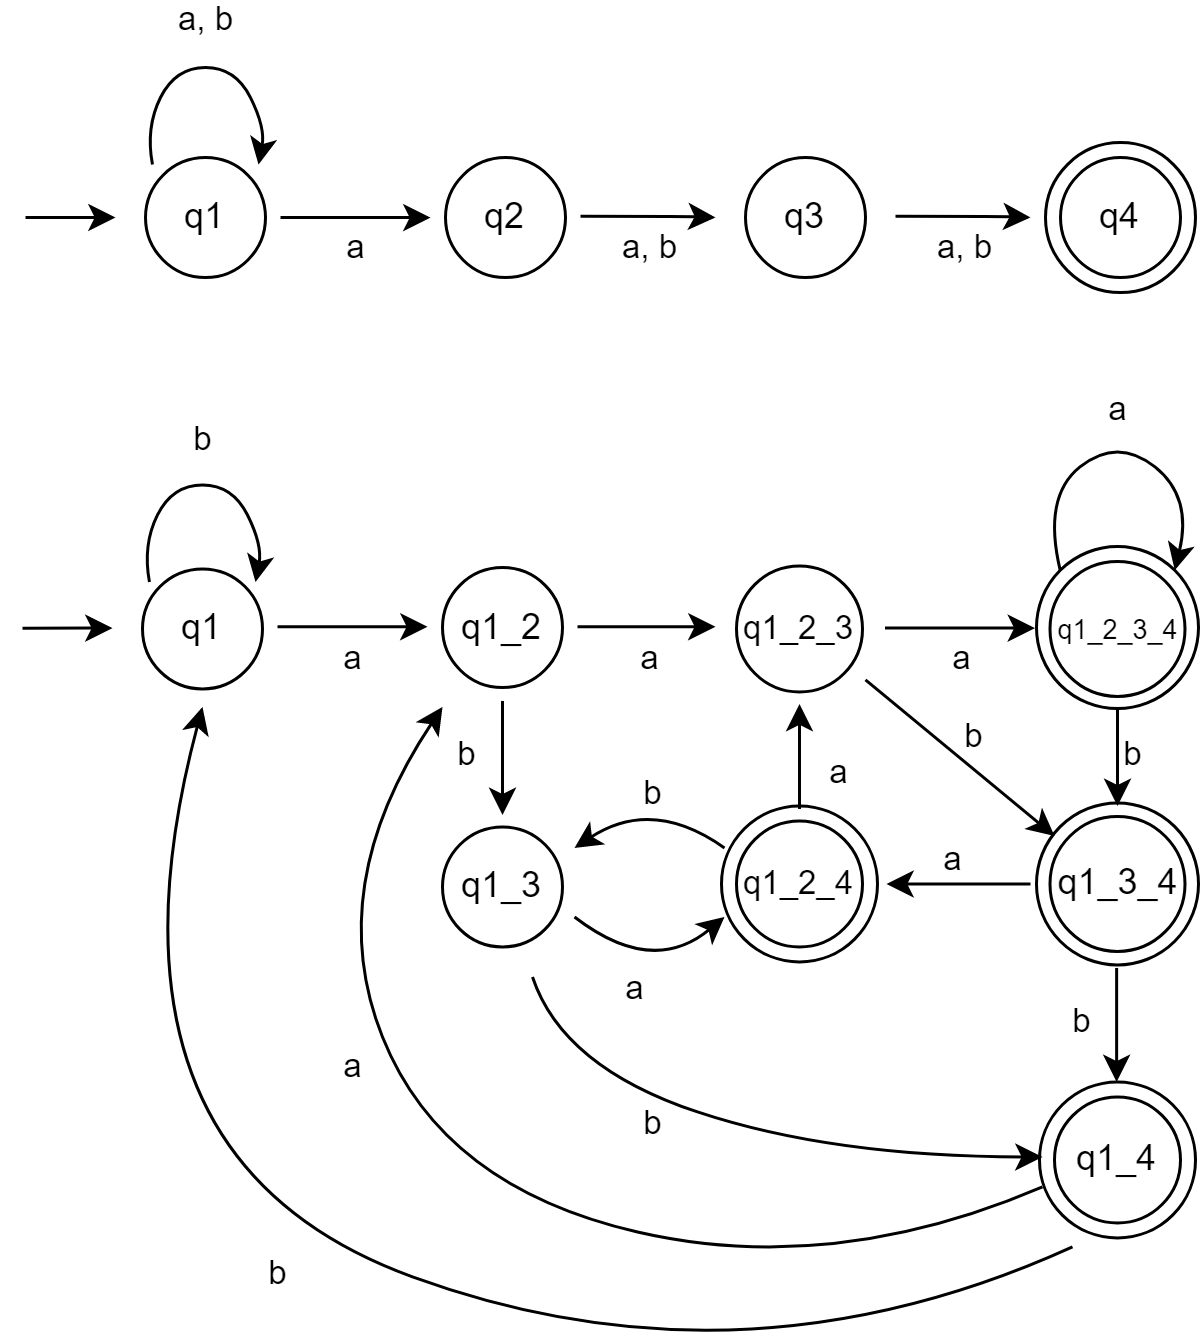
\includegraphics[width=0.6\linewidth]{obrazky-figures/NFA to DFA.drawio.png}
    \caption{On the top is a nondeterministic automaton with four states representing the language $L_{NFA}=(a+b)^*a(a+b)^2$. On the bottom, we can find a deterministic automaton representing the same language with eight states. Even though this DFA is not minimal, we can see the obvious difference in the size of the automata and the simplicity that NFAs offer.}
\end{figure}
\vspace{0.3cm}

 Due to the possibility of numerous transitions for NFAs leading from a single state for a given symbol, they can be more compact and require fewer states and transitions than a minimal DFA defining the same language (see Figure \ref{NFA to DFA}). However, algorithmic work needs a way to comprehend multiple paths for a single word, which is usually done by creating multiple instances of a run for the input word, each trying a different path. Together with the problem of efficient minimization, the use of DFAs is not much lower than that of NFAs as it may seem at first for their theoretically larger size.

\subsection*{Finite State Automaton without unreachable states}
An \textbf{unreachable state} is any state in the automaton described as having no path leading to it starting from an initial state,
\begin{equation*}
    \text{state \textit{p} is unreachable} \iff \nexists q_1 \xrightarrow{a_1} q_2 \xrightarrow{a_2} \dots \xrightarrow{a_n} q_{n+1}: q_1 \in I \land q_{n+1} = p,
\end{equation*}
where $q_1, \dots ,q_{n+1} \in Q, a_1,\dots,a_n \in \Sigma$. As these states are not reachable, they do not affect the function of the automaton and can be simply removed without any extra adjustments in the automaton. 

FSA without unreachable states is an automaton that does not have any of these states.

\subsection*{Complete Deterministic Finite State Automaton}
A \textbf{complete DFA} is a type of deterministic finite state automaton without unreachable states for which it holds that
\begin{equation*}
    \forall p \in Q\forall a \in \Sigma \exists q \in Q: p \xrightarrow{\text{$a$}} q \in R,
\end{equation*}

meaning that for each symbol there exists exactly one transition from each state. As there is a possibility that some states may not have transition leading from them for every symbol, a special type of state is added called the sink state. 

A \textbf{sink state} is a non-accepting state that loops within itself for every symbol of the alphabet meaning that there does not exist any path leading out from the sink state. Any transitions that were missing in the automaton will now be going to the sink state of the complete DFA. This ensures that the input word will be rejected without taking into account the rest of the word.

In our work, we expect every DFA to be a complete DFA unless it is stated otherwise.

\subsection*{Complement Automaton}
The \textbf{complement automaton} $C(M)=(Q_C, \Sigma, R_C, I_C, F_C)$ to nondeterministic automaton $M=(Q, \Sigma, R, I, F)$ is an automaton that defines a~complement language to the original one, formally
\begin{equation*}
    L_C=\Sigma^*-L,\\
\end{equation*}
where $L_c$ is the language of the complement automaton $C(M)$, $L$ language of the original automaton $M$ and $-$ represents the difference between sets. That means that every word that the automaton $M$ accepts is rejected by the automaton $C(M)$ and vice versa.
The most common way of creating a complement automaton is to first create a complete DFA (see Section \ref{ssec:num2.4}) followed by a swap of the final states to the non-final states, as shown by the equation:
\begin{equation*}
    F_c = Q-F
\end{equation*}
An example of the construction of the complement to the given complete DFA can be seen in Figure \ref{compl-rev}.

\begin{figure}[ht]
    \label{compl-rev}
    \centering
    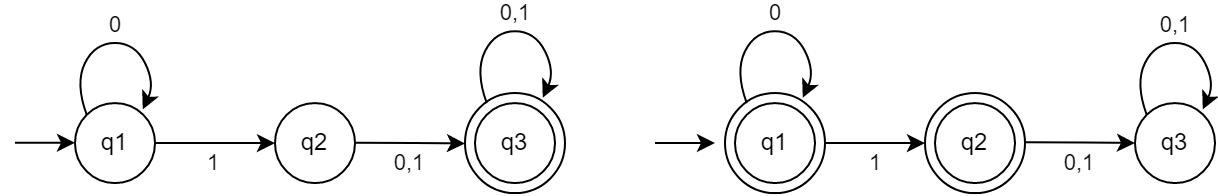
\includegraphics[width=0.9\linewidth]{obrazky-figures/complement.drawio.png}
    \caption{On the left is presented an example of a complete deterministic automaton to which was constructed its complement automaton on the right.}
\end{figure}
\vspace{0.3cm}


\section{Determinization}
\label{ssec:num2.4}
Even though it may seem that NFAs are more powerful than DFAs, that is not the case. The Rabin-Scott theorem says the following~\cite{ Blais2021, Kline2004}:
\begin{quote}
    ``The set of languages that can be recognized by DFAs is exactly the same as the set of languages that can be recognized by NFAs.''
\end{quote}
That means that for every NFA, there exists a DFA defining the same language.

\textbf{Determinization} is a process of transforming an NFA into a language-equivalent DFA. The main idea of this process is to simulate all possible paths in an NFA on the given input simultaneously. This is accomplished by each state of a DFA representing a set of NFA states that the NFA would be in after reading an input word.

Let $M_{NFA}=(Q,\Sigma,R,I,F)$ be an NFA. Then we can define the DFA created by determinization as $M_{DFA}=(Q', \Sigma, R', I', F')$ where:

\begin{itemize}
    \item $Q'$ is a non-empty subset equal to the collection of all subsets of $Q$,  $Q'=P(Q)$,
    \item $R'$ is a transition function in a form of $Q'\times \Sigma \rightarrow Q'$ for which it holds that
    \begin{equation*}
        \forall q' \in Q', a \in \Sigma : R'(q',a) = \cup_{q \in q'} R(q,a),
    \end{equation*}
    \item $I'$ is a set with a single state $I'=\{I\}$, and
    \item $F'$ is a set of states from $Q'$, in which at least one element is an accepting state in automaton $M_{NFA}$, $F' =\{P \subseteq Q \mid P \cap F \neq \emptyset\}$.
\end{itemize}

Generally, determinization consists of two steps, which are the removal of epsilon transitions and the modification of automaton to replace multiple transitions from a single state.
\vspace{2.5mm}

Removal of epsilon transitions can be done through epsilon closures. An \textbf{epsilon \mbox{closure}} of a state $q$, marked as  $\varepsilon_{c}(q)$, is a set of states that can be reached from the state $q$ using exclusively epsilon transitions,
\begin{equation*}
    \varepsilon_{c}(q) = \{p \in Q \mid q \xrightarrow{\varepsilon}^{*} p \},
\end{equation*}
where $\xrightarrow{\varepsilon}^{*}$ represents zero or more consecutive epsilon transitions. In Figure \ref{eps_closure} is shown a visualization of an epsilon closure for each state.

\begin{figure}[ht]
    \label{eps_closure}
    \centering
    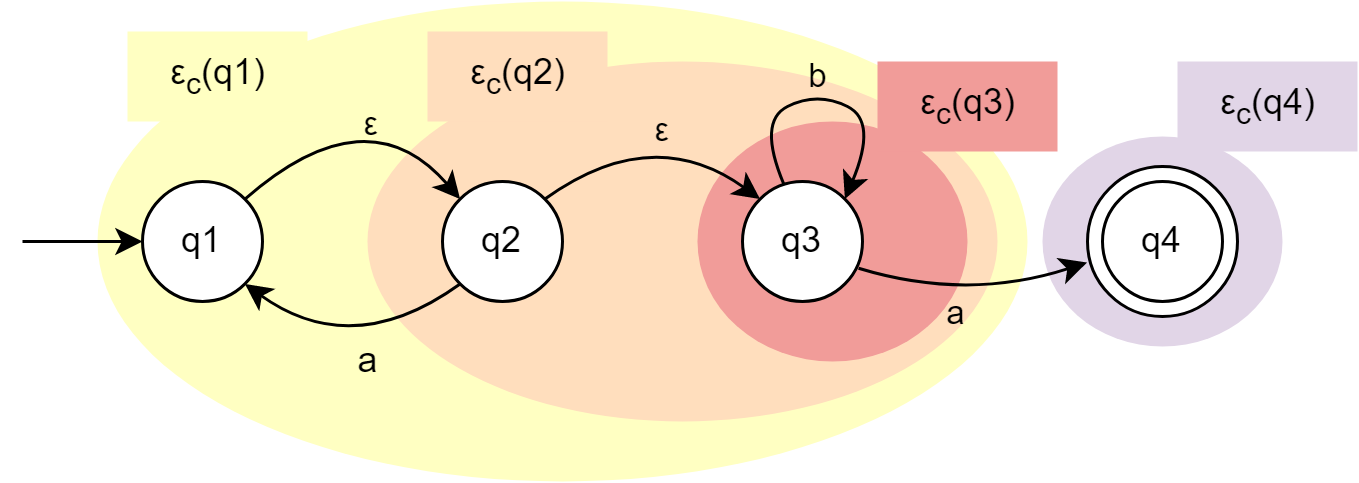
\includegraphics[width=0.7\linewidth]{obrazky-figures/eps_closure.drawio.png}
    \caption{An example of epsilon closures in an automaton. Each closure contains at least the state it belongs to. For state $q2$ we can see that the closure expands onto the state $q3$ because of the epsilon transition $q2\xrightarrow{\epsilon}q3$. Similarly we can see $\epsilon_c(q1)$ spreading to the states $q2, q3$.}
\end{figure}
\vspace{0.3cm}

The epsilon transitions can be removed once the epsilon closures of the automaton's states are noted, and each state must be adjusted so that it can perform all the transitions of every state in its closure without taking into account epsilon transitions anymore. Let $M_{\varepsilon}=(Q, \Sigma, R_\varepsilon, I, F_\varepsilon)$ be $M_{NFA}$ without epsilon transitions. Then we can say that

\begin{equation*}
    \forall q \in Q\forall a \in \Sigma \forall e \in \varepsilon_c(q): e\xrightarrow{a}p \in R \implies q\xrightarrow{a} p \in R_{\varepsilon}
\end{equation*}
Lastly, if a state has as least one accepting state in its epsilon closure then that state is set as an accepting state as well.
\begin{equation*}
    \forall q \in Q: \varepsilon_{c}(q) \cap F \neq \emptyset \implies q \in F_\varepsilon
\end{equation*} 

\begin{figure}[ht]
    \label{eps_rem}
    \centering
    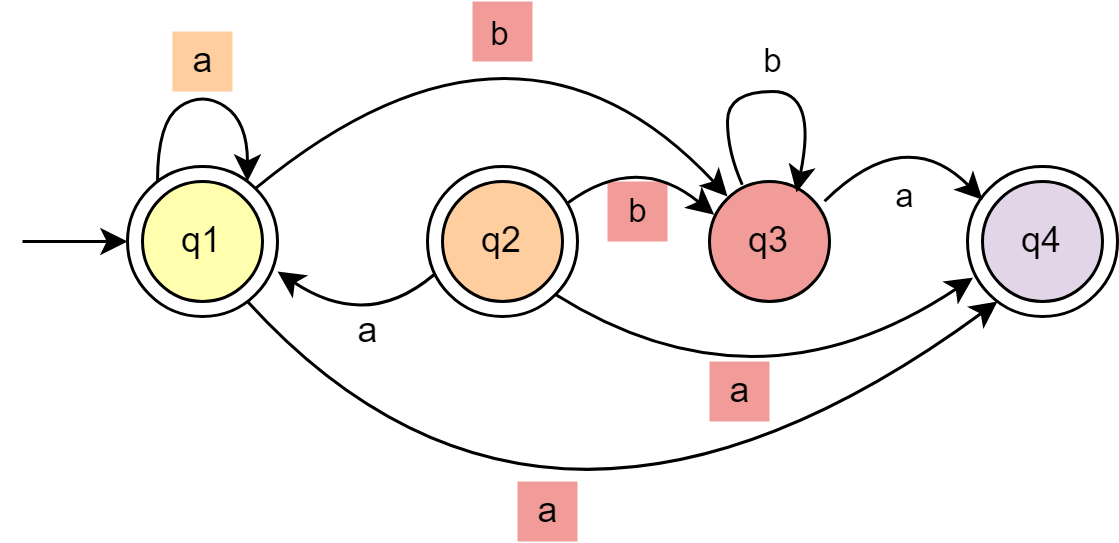
\includegraphics[width=0.7\linewidth]{obrazky-figures/eps_replaced.drawio.png}
    \caption{Automaton from Figure \ref{eps_closure} after the removal of epsilon transitions. Newly created transitions are marked with the color of the state from which the transition was taken. In this case, the looping transition in the state \textit{q1} was originally from the state \textit{q2}. All of the other transitions are duplicates of transitions from \textit{q3}. As an accepting state \textit{q2} was part of $\epsilon_c(q1)$, state \textit{q1} has to be set as an accepting state also.}
\end{figure}
\vspace{0.3cm}

\pagebreak
After the removal of epsilon transitions (see Figure \ref{eps_rem}), we can create a complete DFA $M_{DFA}$ with the same language as the NFA $M_{NFA}$ by the following set of rules:

\begin{enumerate}
    \item The single initial state $s' \in I'$  is created as the set of all initial states of automaton $M_\varepsilon$, $s'=\{I\}$.
    \item Each newly created state $q' \in Q'$ inherits all of the transitions of the states in its set. Let $|R(q,a)|$ be the sum of all transitions for every state $q \in q'$ and symbol $a \in \Sigma$, then three cases can occur:
    \begin{itemize}
        \item $|R(q, a)| = 0$ -- transition to the sink state is added,
        \item $|R(q, a)| = 1$ -- transition $R(q', a) = R(q, a)$ is added, and
        \item $|R(q, a)| > 1$ -- a new state $p'$ is created in the automaton $M_{DFA}$ as a set of all states that the transitions led to $p' = \cup_{q \in q'} R(q, a)$, and the  transition $q' \xrightarrow{a} p' \in R'$ is added.
    \end{itemize}
    \item A state $q$ is set as an accepting state if at least one of the states in its set was accepting, $\forall q \in Q': q \cap F \neq \emptyset \implies q \in F'$.
\end{enumerate}

By applying these rules we will get a complete DFA as seen in Figure \ref{done_det}.

\begin{figure}[!hbt]
    \label{done_det}
    \centering
    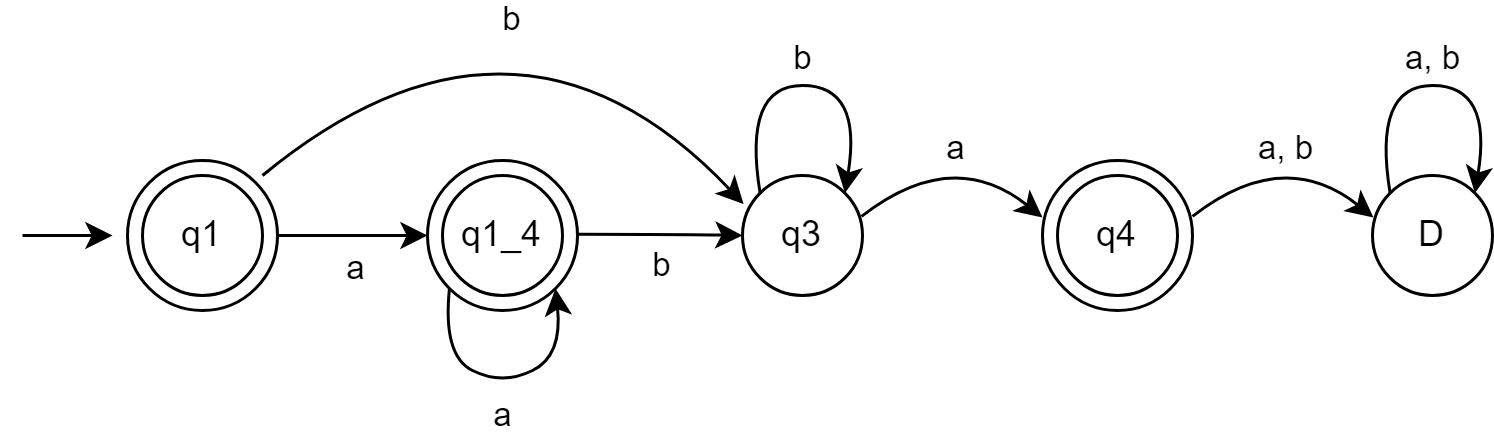
\includegraphics[width=0.8\linewidth]{obrazky-figures/done_deter.drawio.png}
    \caption{Finished determinization of the automaton from Figure \ref{eps_rem}. Two transitions through symbol $a$ from state $q1$ were merged into one leading to the new state $q1\_4$ representing two states $q1$ and $q4$ at once. State D denotes the sink state for the completeness of the DFA.}
\end{figure}
\vspace{0.3cm}

Determinization is a convenient transformation generally used for various operations with the automaton as determinism is often a wanted property for algorithmic tasks. The inevitable part of determinization is the possible exponential increase in the size of the automaton (see Figure \ref{NFA to DFA}).

\section{Propositional Logic}
\label{sec:prop_logic}

\subsection*{Boolean Algebra}
Boolean algebra is a way of describing a system using only two values, \textit{true} (1) and \textit{false} (0), also called \textit{Boolean values}. Let $p$ be variables that store these values. \textbf{Literals} are then the variables themselves or their negations, $\neg p$. The fundamental  Boolean operators are negation ($\neg$), conjunction ($\land$), disjunction ($\lor$), and implication ($ \Rightarrow$). Then we can define a \textbf{propositional formula} as a set of variables connected through Boolean operators. \\

A formula is said to be \textit{satisfiable} if there is at least one combination of input values for which the formula returns the value \textit{true}. Otherwise, it is \textit{unsatisfiable}.

\subsection*{Conjunctive and Disjunctive Normal Form}
A formula is in the \textbf{conjunctive normal form} (CNF), if it consists of a conjunction of \textbf{clauses} and each clause is a disjunction of literals.

Similarly, we can define a \textbf{disjunctive normal form} (DNF). A formula is in DNF, if it contains a disjunction of clauses, each being a conjunction of literals.

These forms set a standard in propositional logic often required as an input format for certain tools and applications.

\subsection*{SAT problem}
The \textbf{Boolean satisfiability} (SAT) \textbf{problem} asks whether the provided formula is satisfiable. The formula is expected to be in a CNF as it was considered more optimal for solving using SAT solvers. SAT problems can be frequently found in mathematics and computer science, which is why the popularity of SAT solvers rises. 
\subsection*{QBF problem}
The \textbf{QBF problem}, much like the SAT problem, questions whether the given formula in CNF is satisfiable. However, the formula can be \textit{quantified}, meaning that it may contain quantified variables. \textit{Quantifiers} are operators used for representing the scope of values of the variables that have to satisfy the formula. There are two types of quantifiers:  $\forall$ -- universal (for all possible values) and $\exists$ -- existential (for a single value).

\subsection*{Transformation to CNF}
When it comes to algorithmic solving, the CNF is the preferred format. Usually, the acquired formula is initially not in CNF; instead, a transformation is required.
The most straightforward method of transformation is by using De Morgan's and distribution laws. They are typically used to modify the form of the clause without affecting its function.

The \textbf{distribution laws} for logical operators work on the same principles as those for addition and multiplication and come in the following forms:
\begin{equation*}
    A \lor (B \land C) \iff (A \lor B) \land (A \lor C) 
\end{equation*}
\begin{equation*}
    A \land (B \lor C) \iff (A \land B) \lor (A \land C)
\end{equation*}

These rules allow changing the operator at the top level by shifting the nested operator that was enclosed in the parenthesis outward, as can be seen above.
\textbf{De Morgan's laws} cover the negation of the conjunction and disjunction and the negation of quantified formulas.
\begin{equation*}
    \neg (A \land B) \iff (\neg A \lor \neg B)
\end{equation*}
\begin{equation*}
   \neg (A \lor B) \iff (\neg A \land \neg B)
\end{equation*}

\begin{equation*}
   \neg \forall x P(x) \iff \exists x \neg P(x) 
\end{equation*}
\begin{equation*}
   \neg \exists x P(x) \iff \forall x \neg P(x) 
\end{equation*}
\\
By a combination of these laws, we can gradually convert the given formula into the CNF. Let $(A \land B \land C) \lor \neg (D \lor E)$ be the input formula, then a step-by-step conversion could go as follows:
\begin{align*}
    (A \land B \land C) \lor \neg (D \lor E) =& (A \land B \land C) \lor (\neg D \land \neg E)=\\
    =& (A \lor (\neg D \land \neg E)) \land (B \lor (\neg D \land \neg E)) \land (C\lor (\neg D \land \neg E)) =\\
    =& (A \lor \neg D) \land (A \lor \neg E) \land (B \lor \neg D) \land (B \lor \neg E) \land {}\\ &\land (C\lor \neg D) \land (C \lor \neg E)
\end{align*}

This technique works for smaller clauses but has exponential growth of the final formula. This property is not suitable for efficient usage of the solvers and should be avoided. \\

The different method of obtaining an equivalent CNF formula is by using the \textbf{Tseytin transformation}. The algorithm involves creating new variables as placeholders to represent sub-clauses in the formula. It utilizes the combinational logic when each sub-clause can be represented as a gate that can be expressed as a formula in CNF. All gates are combined to form a circuit. By setting the output of the circuit to value 1, the solver can work backward to get the values of the original variables on the input. Despite the need for more variables, the overall number of clauses decreases for more complex formulas compared to conversion utilizing only De Morgan's and distribution laws. \\

The example clause $(A \land B \land C) \lor \neg (D \lor E)$ can be represented by a circuit shown in Figure \ref{fig:tsey}. We establish new variables $X, Y, W, Z$ for the output of each gate that serves as its representation in subsequent processes. Lastly, the output of the entire circuit $Z$ is set to be true.

\begin{figure}[ht]
    \label{fig:tsey}
    \centering
    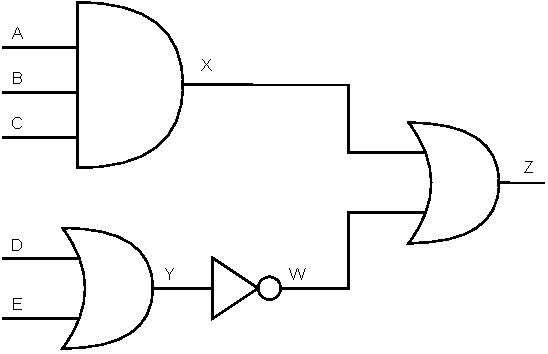
\includegraphics[width=0.5\linewidth]{obrazky-figures/tseytin_diagram.drawio.pdf}
    \caption{Circuit representation of the example clause $(A \land B \land C) \lor \neg (D \lor E)$. Each sub-clause is represented as a logical gate corresponding to its function.}
\end{figure}
\vspace{0.3cm}

In this instance, it is possible to create a truth table for each gate, which can be used for the transformation into a clause in CNF. The truth table contains every combination of literals of input and output variables. The \textit{Result} column references whether the operation of the gate on the values of the input variables results in the value on the output (marked with value 1) or not (marked with value 0). The formula in CNF is then obtained by creating a conjunction of clauses where each clause is a \textit{negation} of every row for which the result is false. The \textit{negation} of the row refers to creating a disjunction of negated literals on the specified row. The truth table for \textit{OR} joined with the \textit{NOT} operation as well from the circuit in Figure \ref{fig:tsey} is shown in Table \ref{tab:truth_table}.


\begin{table}[!hbt]
    \centering
    \label{tab:truth_table}
    \caption{Truth table for the \textit{OR} gate from Figure \ref{fig:tsey} used for transformation into CNF.}
    \vspace{0.3cm}
    \begin{tabular}{|c||c|c|c||c|} \hline
         \textbf{Row} &\textbf{D} & \textbf{E} & \textbf{W} & \textbf{Result}
           \\ \hline \hline
         1. &   0    &   0   &   0   &   0 \\ \hline
         2. &   0    &   0   &   1   &   1 \\ \hline
         3. &   0    &   1   &   0   &   1 \\ \hline
         4. &   0    &   1   &   1   &   0 \\ \hline
         5. &   1    &   0   &   0   &   1 \\ \hline
         6. &   1    &   0   &   1   &   0 \\ \hline
         7. &   1    &   1   &   0   &   1 \\ \hline
         8. &   1    &   1   &   1   &   0 \\ \hline
    \end{tabular}
\end{table}

The following formula contains a clause for each of the false rows (with numbers 1, 4, 6, and 8 in Table \ref{tab:truth_table}) in the corresponding order.
\begin{equation*}
    (D \lor E \lor W) \land (D \lor \neg E \lor \neg W) \land (\neg D \lor E \lor \neg W) \land (\neg D \lor \neg E \lor \neg W)
\end{equation*}

This formula be further optimized to find its shortest possible version, which is shown in Equation \ref{eqn:2.2} below. 

The whole circuit can be then represented by three clauses in CNF, which are a clause for \textit{AND} gate (\ref{eqn:2.1}), for \textit{OR} and \textit{NOT} gate combined utilizing the De Morgan's law (\ref{eqn:2.2}), and a clause for the final \textit{OR} gate also with setting the output to value true (\ref{eqn:2.3}).

\begin{equation}
\label{eqn:2.1}
   (A \lor \neg X) \land (B \lor \neg X) \land (C \lor \neg X) \land (\neg A \lor \neg B) \land (\neg C \lor X)
\end{equation}
\begin{equation}
\label{eqn:2.2}
    (\neg D \lor \neg W) \land (\neg E \lor \neg W) \land (D \lor E \lor W)
\end{equation}
\begin{equation}
\label{eqn:2.3}
    (\neg X \lor Z) \land (\neg W \lor Z) \land (X \lor W \lor \neg Z) \land Z
\end{equation}


\chapter{Known Reduction Algorithms for FSAs}
\label{chap:reduction}
This chapter will outline the various methods of automata reduction that were implemented and tested in the thesis. We can divide these reductions into two sections. The first section presents the reduction of deterministic automata through various methods of finding the minimal DFA. As this kind of reduction has consistent results, it can represent a baseline for comparison with other reductions. In the second section, we will discuss selected types of nondeterministic reduction.


\section{DFA Reduction}
\textbf{DFA minimization} is a process of finding the smallest deterministic automaton equivalent to the given one. Such a minimized automaton is unique except for isomorphisms. Even though there exist multiple algorithms for DFA reductions, their output will always be the same minimal DFA. If the input automaton is an NFA, it must be determinized first. Generally, the reduction consists of two steps:
\begin{enumerate}
    \item Removing any unreachable and potential sink states (except the sink state required for the completeness of a DFA).
    \item Merging indistinguishable, equivalent states of the automaton \cite{TIN}.
\end{enumerate}

Two states $q_1,p_1 \in Q$ are considered \textit{equivalent} in automaton $M=(Q, \Sigma, R, I, F)$ if the following holds
\begin{equation*}
    \forall a_1 a_2...a_n \in \Sigma^{*}: q_1 \xrightarrow{a_1} \dots \xrightarrow{a_n} q_{n+1} \land q_{n+1} \in F \iff p_1 \xrightarrow{a_1} \dots \xrightarrow{a_n} p_{n+1} \land p_{n+1} \in F,
\end{equation*}
which means that for every input word, the path from state $q_1$ ends up in an accepting state only if the path from state $q_2$ for the same word ends in an accepting state as well. As these states have the same behavior for all the inputs, they can be merged and represented as one.

In our work, we looked at two algorithms of DFA minimization: Hopcroft’s and Brzozowski’s algorithms. We expect that the input automaton had already had the extra unreachable and sink states removed.

\subsection{Hopcroft's Algorithm}
In the article \cite{Hopcroft1971} from 1971, John Hopcroft presented his new algorithm for DFA minimization. It was the first algorithm that in the worst case runs in the asymptotic time $O(n\log n)$ (as opposed to by then-known best algorithms running at $O(n^2)$), where $n$ is the number of automaton states.
This makes Hopcroft’s algorithm used until these days, still recognized as one of the most efficient and reliable reduction algorithms for DFAs \cite{Gracia, Paun2009}.

Hopcroft’s algorithm works by dividing the set of states into partitions based on how each partition responds to the input with respect to the other partitions. These equivalence partitions are refined until a fixpoint. States with the same behavior end up in the same partition so that they can be merged into a single state and transitions leading from this state are equal to the behavior of the whole partition. The entire reduction algorithm can be seen in Algorithm \ref{alg:hopcroft}.

\begin{algorithm}
\caption{Hopcroft's algorithm for automata minimization}\label{alg:hopcroft}
 \hspace*{\algorithmicindent} \textbf{Input: } $M_{DFA}=(Q,\Sigma,R,I,F)$\\
 \hspace*{\algorithmicindent} \textbf{Output:}  Minimal $N_{DFA}=(Q',\Sigma,R',I',F')$ \\
 \hspace*{\algorithmicindent} \textbf{Require:}  $M_{DFA}$ does not have any unreachable states
\begin{algorithmic}[1]
\LState $P_{NEW} = \{Q-F, F\}, P_{OLD} = \{\}$
\While{$P_{NEW} \neq P_{OLD}$}
    \LState $P_{OLD} \gets P_{NEW}$
    \LState $P_{NEW} = \{\}$
    \For{$S \in P_{OLD}$}
        \ForAll{$q \in S$}
            \LState found $\gets$ \textit{false}
            \If{$P_{NEW}= \emptyset$}
                \LState $P_{NEW}\gets$\{$q$\}
                \LState \textit{continue}
            \popindent\EndIf
            \For{$S' \in P_{NEW}$}
                \If{$behavior(S', P_{OLD}) = behavior(q, P_{OLD})$}
                    \LState \textit{add} $q$ to $S'$
                    \LState found $\gets$ \textit{true}
                    \LState \textit{break}
                \popindent\EndIf
            \popindent\EndFor
            \If{\textit{not} found}
                \LState \textit{add} \{$q$\} to $P_{NEW}$
            \popindent\EndIf
        \popindent\EndFor
    \popindent\EndFor
\popindent\EndWhile
\For{$S \in P_{OLD}$}
    \LState \textit{add} $S$ to $Q'$
    \LState \textit{add} $behavior(S, P_{OLD})$ to $R'$
    \If{$S \cap F \neq \emptyset$}
        \LState \textit{add} $S$ to $F'$
    \popindent\EndIf
    \If{$S \cap I \neq \emptyset$}
        \LState \textit{add} $S$ to $I'$
    \popindent\EndIf
\EndFor
\Return
\end{algorithmic}
\end{algorithm}

The algorithm starts with two partitions, one containing all accepting states $F$ and the other containing all non-accepting states $Q-F$. As non-accepting states require an input word of the length of at least one in order to reach a final state, we can conclude that the states in these two partitions are not language-equivalent. For each state in every partition, we look at its \textit{behavior} across all symbols with regard to the existing partitions $P_{OLD}$ (line 12). \textit{Behaviors} of two elements are considered equal if the transition through every symbol of the alphabet leads to a state in the same partition. For example, if two states $x$ and $y$ are from the set of non-accepting states and $x$ have a transition through symbol $a$ to a final state while $y$ does not, their \textit{behaviors} differ. If the set $P_{NEW}$ is empty (lines 8-10) or there is no subset in this set with the same \textit{behavior} as the searched state (lines 16-17), the state will create a new subset with this \textit{behavior}. If an element finds a subset with the same \textit{behavior}, it is added to the subset (lines 11-15). In this manner, the partitions will break into subsets, keeping together the states that \textit{behave} identically across all symbols. These subsets will produce new partitions, and this step is repeated until no further splitting is possible. The final partitions represent the new states of the minimal deterministic automaton. In Figure \ref{part_tree} is presented an example of partition splitting for the automaton from Figure \ref{done_det}. 

\begin{figure}[ht]
    \label{part_tree}
    \centering
    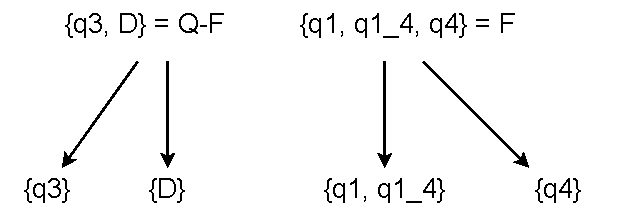
\includegraphics[width=0.55\linewidth]{obrazky-figures/partition_tree.drawio.pdf}
    \caption{Finding the minimal DFA for the automaton from Figure \ref{done_det} through partition splitting. Starting from the sets of accepting and non-accepting states, we check the behavior of each state in the partitions. As state $q3$ goes to a final state while state $D$ does not, they need to be separated. The same applies for $q4$, which for symbol $a$ results in a non-accepting state while states $q1$ and $q1\_4$ end in a final state. As no further splitting is possible, these four partitions represent the states of the minimal DFA.}
\end{figure}
\vspace{0.3cm}

\subsection{Brzozowski's Algorithm}
Brzozowski’s algorithm uses the process of determinization to create the minimal deterministic automaton. It has been proven \cite{Bonchi2012, Gracia} that automaton $M$ can be turned into minimal DFA $M_M$ by determinizing the reverse automaton of $M$ followed by reversion and another determinization, $M_M=D(R(D(R(M))))$  where functions $D(A)$ and $R(A)$ stands for determinization and reversion of automaton $A$ in the corresponding order.

There is no need to determinize the automaton beforehand since it will be done during reduction, hence the input automaton for this algorithm can be an NFA. The efficiency of this reduction depends on the size of the reversed determinized automaton, which could be exponential in the worst case.

\section{NFA Reduction}
On the contrary, there is no known algorithm to successfully and efficiently find the smallest nondeterministic automaton without enumerating all of the possible automata from the smallest one as the problem of finding the minimal NFA for the given language is PSPACE-complete. There are still new ways of direct reduction of NFAs being researched. In our work, we looked at two reduction ideas whose concept is based on using the simulation relation and transformation into a canonical residual automaton.

\subsection{Reduction using the Relation of Simulation}
In the article \textit{On NFA Reductions} \cite{Ilie2004} there has been introduced reduction using the simulation relation named an \textit{NFA reduction using preorders}.

\textbf{Simulation} is a reflexive and transitive binary relation between states of the automaton. Let $\preceq$ be a symbol for simulation and $M_{NFA}=(Q,\Sigma, R, I, F)$ be a nondeterministic automaton. According to the definition, state $q$ is simulated by state $p$ if it holds that for each transition from state $q$ to $q'$ there must be a transition from state $p$ to state $p'$ such that state $q'$ is once again under the relation of simulation of state $p'$ and if state $q'$ is an accepting state then the state $p'$ must be an accepting state also, formally

\begin{equation*}
    q \preceq p \implies \forall a \in \Sigma , q\xrightarrow{\text{$a$}}q' \in R \exists p\xrightarrow{\text{$a$}}p' \in R: q' \preceq p' \land (q \in F \implies p \in F) 
\end{equation*}
where $q,q',p,p' \in Q$. As it is apparent from the definition that two pairs of states cannot be simulated. Firstly it is a pair of accepting and non-accepting states (similar to the equal states in Hopcroft’s algorithm) and secondly, the pair of states, which have at least one transition for a symbol while others do not. From there, it is possible to work backward to search for all the states where the simulation's relationship was severed. After the computation of the relation is complete, its \textit{symmetric fragment} (to ensure that both states are simulating each other simultaneously) is used to find the groups of states that can be merged and represented as one.

\begin{algorithm}
\caption{Computation of the simulation relation} \label{alg:simulation}
 \hspace*{\algorithmicindent} \textbf{Input: } $M_{NFA}=(Q,\Sigma,R,I,F)$\\
 \hspace*{\algorithmicindent} \textbf{Output:} Simulation relation
\begin{algorithmic}[1]
\LState que = new\_queue(), card\_tables
\LState init whole $\omega[N][N]$ with value true
\Comment{$N = Q.size()$}
\LState $M_R \gets reverse(M_{NFA})$
\For{$q\in Q, a \in \Sigma$}{}
    \LState $card\_tables_{a}[q] \gets fill\_row(card(R(q,a)))$
\popindent\EndFor
\For{$q \in Q$}
    \If{$q \notin F$}
        \For{$f \in F$}
            \If{$\omega[f][q] = true$}
                \LState $\omega[f][q] \gets false$
                \LState \textit{push\_back}(que, $(f,q)$)
            \popindent\EndIf
        \popindent\EndFor
    \popindent\EndIf
    
    \For{$p \in Q, a \in \Sigma$}
        \If{$card(R(q,a) \neq$ 0 and card(R(p, a)) = 0 \textit{and} $\omega[q][p]$ = \textit{true}}
            \LState $\omega[q][p] \gets$ \textit{false}
            \LState \textit{push\_back}(que, $(f,q)$)
        \popindent\EndIf
    \popindent\EndFor
\popindent\EndFor
\While{\textit{not} \textit{empty}(que)}
    \LState $(i,j)$ $\gets$ \textit{pop\_back}(que)
    \For{$a \in \Sigma$}
        \LState $k\_trans \gets get\_trans(M_{R}, j)$
        \For{$k \in k\_trans$}
            \LState $card\_tables_{a}[k][i] = card\_tables_{a}[k][i] - 1$
            \If{ $card\_tables_{a}[k][i] = 0$}
                \LState $m\_trans \gets get\_trans(M_{R}, i)$
                \For{$m \in m\_trans$}
                    \If{$\omega[m][k] = true$}
                        \LState $\omega[m][k] \gets false$
                        \LState  push\_back(que, $(m,k)$)
                    \popindent\EndIf
                \popindent\EndFor
            \popindent\EndIf
        \popindent\EndFor
    \popindent\EndFor
\popindent\EndWhile
\LState \textit{return} $\omega$
\end{algorithmic}
\end{algorithm}

A simulation relation is represented by a 2D array of size $n\times n$, where $n$ is the number of automaton states. The value of a cell $(i,j)$ indicates whether the state $i$ is being simulated by the state $j$. We expect that all states are simulated by each other at first (line 4). Gradually the pairs of states $(i,j)$ will lose their \textit{status of simulation} (state $i$ is not being simulated by $j$) and will be added to the queue for later measures. Variable \textit{card\_tables} holds for each state and symbol the number of transitions to simulated states. As the states are found not being simulated, the number of transitions will decrease (line 20). If it reaches zero, such a state does not have any simulated states to transition to and the relation will break further. After the queue is empty, the simulation relation can be utilized for automata reduction. The whole process of computing the relation of simulation for the given automaton can be seen in Algorithm \ref{alg:simulation}.

The effectiveness of this type of reduction solely depends on the constructed relation, which in the worst-case scenario, does not have to reduce the automaton at all. However, it is impossible for the reduced automaton to have more states than the original one.

\pagebreak
\subsection{Reduction using Residual Automata}

A different method of nondeterministic reduction was introduced in the article \textit{Residual Finite State Automata} \cite{Denis2001}. The idea of this reduction was to construct a canonical residual automaton from a given one, which in the worst-case scenario has the same number of states as the minimal deterministic automaton. 

\textbf{Residual automaton} (RSA) $M_{RSA}=(Q, \Sigma, R, I, F)$ is defined as a type of NFA that in every state classifies a \textit{residual language} of the automaton language

\begin{equation*}
{\forall q \in Q, \exists u \in \Sigma^*: L_q = u^{-1}L_M},
\end{equation*}

where $L_q$ is the language of state q and $L_M$ is the automaton language.

A \textbf{residual language} $L$ with regard to a prefix $u \in \Sigma^*$ is described as 

\begin{equation*}
{u^{-1}L = \{v \in \Sigma^*|uv \in L\}}
\end{equation*}

From this definition, it can be stated that every DFA is also an RSA, but it does not apply vice versa.

\textbf{Canonical residual automaton} (CRSA) is the RSA with a minimal number of states. \\

The construction of a residual automaton can be divided into two steps. The first step is identical to the determinization using the subsets to create a DFA with the same language as the given NFA. Let ${M_{NFA}=(Q, \Sigma, R, I, F)}$ be an input NFA and let \linebreak ${M_{DFA}=(Q_{DFA}, \Sigma, R_{DFA}, I_{DFA}, F_{DFA})}$ be language equivalent DFA created by deteminization, with $Q_{DFA}=\{p \in P(Q) \mid \exists a_1,\dots,a_n \in \Sigma: q_1 \xrightarrow{a_1} \dots \xrightarrow{a_n} p \land q_1 \in I' \}$, where $P(Q)$ the collection of all subsets of $Q$. The main focus of the second step is to remove \textbf{coverable states}. State $q \in Q_{DFA}$ is \textit{coverable} if there exists a union of states $q_i$ that is equal to the state $q$ without including the state itself,

\begin{equation*}
\text{state \textit{q} is coverable} \iff \exists q_i \in Q_{DFA}: q = \cup_{i} q_i \land q \neq q_i
\end{equation*}

If the state is coverable, it may be removed from the automaton along with the transitions leading from this state. All of the transitions going into this state must be redirected to every state $q_i$ that is covering the state $q$.

\begin{algorithm}
\caption{Reduction by creating canonical residual automaton} \label{alg:residual}
 \hspace*{\algorithmicindent} \textbf{Input: } $M_{NFA}=(Q,\Sigma,R,I,F)$\\
 \hspace*{\algorithmicindent} \textbf{Output:}  Canonical $N_{RSA}=(Q',\Sigma,R',I',F')$ \\
 \hspace*{\algorithmicindent} \textbf{Require:}  $M_{NFA}$ is reversed determinized 
\begin{algorithmic}[1]
\LState $Q_{NEW} = \{I\}, R_{NEW} = \{\}$
\For{\textit{new} $q \in Q_{NEW}$, $a \in \Sigma$}
    \LState $N = \{\}$
    \For{$r_{qap} \in R$}
        \LState \textit{add} $p$ to $N$
    \popindent\EndFor
    \If{ \textit{count}($N$, $Q_{NEW}$) = 0}
        \LState \textit{add} $N$ to $Q_{NEW}$
        \LState $R_{NEW}(N,a) \gets \cup R(q,a)$
    \popindent\EndIf
\popindent\EndFor
\LState $N_{RSA} \gets (Q_{NEW}, \Sigma, R_{NEW}, \{I\}, F_{NEW})$
\Comment{$F_{NEW} \gets Q_{NEW} \cap F$}
\For{$p \in Q_{NEW}$}
    \For{$C \in P(Q_{NEW})$}
        \If{p \textit{is\_coverable} by $C$}
            \For{$r_{qap} \in R_{NEW}$}
                \For{ $c \in C$}
                    \LState \textit{add} $r_{qac}$ to $R_{NEW}$
                    \popindent\EndFor
                \LState \textit{remove} $r_{qap} $ from $ R_{NEW}$
            \popindent\EndFor
            \LState \textit{remove} $q$ from $N_{RSA}$
        \popindent\EndIf
    \popindent\EndFor
\popindent\EndFor
\end{algorithmic}
\end{algorithm}

The whole process of reduction can be seen in Algorithm \ref{alg:residual} that takes a reverse determinized NFA as an input and outputs a CRSA. The algorithm starts with a process of determinization (lines 2-8) followed by checking for \textit{coverable} states. If state $p$ is coverable by a set of states $C$, every transition leading to state $p$ will be redirected to every state covering this state $p$ (lines 13-16). After this measure, the \textit{covered} state $p$ can be removed. This automaton in the worst case has the same number of states as the minimal DFA for the language of the automaton.

The process of creating a CRSA involves running the algorithm for the construction of residual automaton two times, firstly backward and then forward. Because every DFA describes a residual language, we can use the determinization of reverse automaton as a simpler way to get an automaton with a reverse residual language. The downside of this algorithm may be the unexpected expansion during the determinization. Those states will eventually be removed as they will be covered so the result automaton will not be affected in its size. However, the algorithm may take time to compute with a larger structure than would be anticipated.

\chapter{Reduction Utilizing SAT and QBF Solvers}
\label{chap:sat_qbf}

SAT and QBF solvers are rather powerful tools that were optimized to efficiently solve the problem of whether there exists an assignment to variables of a propositional formula in CNF that would satisfy it. Exhaustive solving of this NP-complete problem would entail attempting every combination of values that the variables may hold. Yet, the fact that SAT solvers can handle a huge number of variables and clauses has increased their appeal in the field of information technology \cite{GaneshV20, Masina2023}. We search for a way to encode an automaton with the given number of states defining the specific language as a formula in CNF solvable by the solvers and utilize it to reduce NFAs.

Every automaton can be precisely characterized by its number of states, the number of symbols of its alphabet, and the language it is defining. The first two conditions can be represented as a pair of constant numbers, $N$ for the number of states and $|\Sigma|$ for the number of symbols of the alphabet. For the representation of the language of the automaton, we worked with the concept of sample words that would shape the language of the final automaton. We constructed two sets of words \textit{Acc} and \textit{Rej} for the automaton to accept and reject accordingly. These would be updated until the language-equivalent automaton is produced. 

 We created an algorithm for converting these selected arguments into a Boolean logic formula that represents an instance of an automaton with the demanded parameters. Finally, we developed a process of utilizing SAT and QBF solvers to find the automaton described by the input formula to discover its smaller equivalent.

In this chapter, we will look at the proposed rules for generating a CNF formula for SAT solvers representing either a DFA or an NFA. Then, we present rules for QBF solvers with quantified variables used for universal quantification over multiple paths in nondeterministic automata. Lastly, we create an algorithm for FSA reduction utilizing SAT and QBF solvers.

\section{Boolean Representation of FSAs for SAT Solvers}

As already said, SAT solvers take a CNF formula for their input. Firstly, we focused on representing the deterministic automata as a foundation that we could later expand onto nondeterministic automata using quantified variables in QBF solvers.

We did not consider applying these rules for NFA representation because of the large amount of paths in the automaton. As we are defining the automaton language through example words, expressing every possible combination of transitions that a word could take, we did not expect this process to have a high potential. However,  because the rules for generating a formula representing a DFA could be easily adapted to represent an NFA, we implemented this representation for SAT solvers as well to explore its capabilities.

We created a set of four conditions using which we defined the given DFA in Boolean algebra; those conditions are:

\begin{enumerate}
    \item $\boldsymbol{\varphi_{det}}$ -- ensuring that the generated automaton is deterministic
    \item $\boldsymbol{\varphi_{comp}}$ -- ensuring the the generated automaton is complete
    \item $\boldsymbol{\varphi_{acc}}$ -- ensuring that the generated automaton is accepting the word set \textit{Acc}
    \item $\boldsymbol{\varphi_{rej}}$ -- ensuring that the generated automaton is rejecting the word set \textit{Rec}
\end{enumerate}

The construction of the CNF formula for the automaton would then consist of creating a conjunction of the formulas generated by these clauses:

\begin{equation*}
    \varphi_{det} \land \varphi_{comp} \land \varphi_{acc} \land \varphi_{rej}
\end{equation*}

Based on the input parameters, we can ensure that the created automaton will have the requested size while defining the given language. In Section \ref{subsec:NFA per for SAT}, we explain how these conditions were utilized for NFA representation.

\subsection{Determinism of the Automaton}

For deterministic automata, it holds that every state has a maximum of one transition for every symbol of the alphabet as stated in Section \ref{sec:dfa}.

Let $t_{qap}\in R, q,p \in Q $ and $a \in \Sigma$ be all of the potential transitions between states in the given automaton and let variables $T_{qap}$ represent whether the responding transition exists in the automaton. These transitions can be organized and numbered for their representation in the solver as shown in Table \ref{tab:fsa32}.

We call a \textit{section} all transitions leading from a single state over the given symbol, so Table \ref{tab:fsa32} consists of six sections. 
\begin{table}[hb]
\centering
\label{tab:fsa32}
\caption{Ordered transition of the automaton $M$ with $N=3$ and $|\Sigma| = 2$, where $1,2,3 \in Q$ and $a,b \in \Sigma$. The first variable $T_1$ would thus indicate if the automaton has a transition from state $1$ to state $1$ using the symbol $a$, and the last variable $T_{18}$ would correspond to transition $t_{3b3}$.}
\vspace{0.3cm}
\begin{tabular}{ c c c }
 $t_{1a1}$ & $t_{1a2}$ & $t_{1a3}$ \\
 $t_{2a1}$ & $t_{2a2}$ & $t_{2a3}$ \\ 
 $t_{3a1}$ & $t_{3a2}$ & $t_{3a3}$
\end{tabular}
\hspace{1cm}
\begin{tabular}{ c c c }
 $t_{1b1}$ & $t_{1b2}$ & $t_{1b3}$ \\
 $t_{2b1}$ & $t_{2b2}$ & $t_{2b3}$ \\ 
 $t_{3b1}$ & $t_{3b2}$ & $t_{3b3}$
\end{tabular}
\end{table} 

With these transition variables, we can define determinism in the automaton by permitting the existence of at most one transition from each state over a symbol. This property can be described by a set of clauses, each of which is a negated conjunction of two transition variables. In accordance with this, a pair may only have one transition allowed. A new clause will be generated for every possible combination of two transitions for a section meaning that we will have $\binom{N}{2}$ clauses per section, where $N$ is the number of states also representing the number of transitions in one section.

For the automaton $M$ from Table \ref{tab:fsa32}, the formula ensuring determinism of state $0$ would consist of three clauses that are $\neg T_{1a1} \lor \neg T_{1a2}$, $\neg T_{1a1} \lor \neg T_{1a3}$, and $\neg T_{1a2} \lor \neg T_{1a3}$, each with a different transition pair. Generally, for automaton with ordered transitions with $N$ states and $|\Sigma|$ symbols, we generate $N\times|\Sigma|\times\binom{N}{2}$ clauses in CNF following the pattern of creating every possible unique combination of two transitions from a section,
\begin{align*}
    \centering
    \neg T_1 &\lor \neg T_2  && \text{-- combinations for the \nth{1} section}\\
    \neg T_1 &\lor \neg T_3 \\
    & \vdots \notag \\
    \neg T_{N-1} &\lor \neg T_{N} \\
    \neg T_{N+1} &\lor \neg T_{N+2} && \text{-- combinations for the \nth{2} section}\\
    \neg T_{N+1} &\lor \neg T_{N+3} \\
    &\vdots \notag \\
    \neg T_{2N-1} & \lor \neg T_{2N} \\
    & \vdots \notag \\
    \neg T_{(N\cdot |\Sigma|\cdot N)-1} & \lor \neg T_{N\cdot |\Sigma|\cdot N} && \text{-- the last combination for the $N\cdot |\Sigma|$\textsuperscript{th} section}
\end{align*}

\subsection{Completeness of the Automaton}
In order to generate a complete DFA, adding a clause for each section is necessary to secure that a transition from every state for each symbol is present in the automaton. Together with the clauses for determinism, they denote a formula for the DFA with exactly one transition per section. The general form of these clauses is as follows:
\begin{align*}
    \centering
    T_1 \lor T_2 \lor & \dots \lor T_{N} \\
    T_{N+1} \lor T_{N+2} \lor & \dots \lor T_{2N} \\
    T_{2N+1} \lor T_{2N+2} \lor & \dots \lor T_{3N} \\
    & \vdots \notag \\
    T_{((|\Sigma|\cdot N-1)\cdot N) + 1} \lor T_{((|\Sigma|\cdot N-1)\cdot N) + 2} \lor & \dots \lor T_{N\cdot|\Sigma|\cdot N}
\end{align*}

The property of being complete is desired in our approach since it grants the automaton a certain level of uniformity. Creating a complete DFA might result in the automaton having one extra state to act as a sink state that it would have otherwise. These clauses are optional and do not need to be included in the final formula in order for the automaton to form correctly. However, their absence may occasionally result in the generation of the automaton without any transitions at all, depending on the example words describing its language.

\subsection{Acceptance of Words}

The automaton accepts the input word if there is a path from the initial state to an accepting state over the word within the automaton. As a deterministic automaton has precisely one initial state by definition,  thus we establish that state $1$ will always be the initial state. Then we can state that the automaton accepts a word if the two following statements hold:

\begin{enumerate}
    \item There exists a series of transitions over the given symbols starting from the initial state $1$.
    \item The state where the path ends must be an accepting state.
\end{enumerate}

We can satisfy the first premise using the transition variables $T_{qap}$ from earlier sections. For the second statement, we need to introduce new variables $F_1, F_2,\dots, F_N$ that indicate whether the states given by their indices are accepting states or not. Using these variables we can define a formula for accepting a word by the automaton with $N^l$ clauses, where $l$ stands for the length of the input word. Each clause will specify a viable sequence of transitions starting from state $1$ and ending in an accepting state.

Let $abb$ be an example word that the automaton with $N=3$ and $|\Sigma|=2$ should accept. Then we can construct a formula with $N^3$ clauses in DNF accepting this word. These clauses are describing all possible paths in the automaton for the word that ends in an accepting state,
\begin{align*}
    \centering
    T_{1a1} \land T_{1b1} &\land T_{1b1} \land F_1 \\
    T_{1a1} \land T_{1b1} &\land T_{1b2} \land F_2 \\
    T_{1a1} \land T_{1b1} &\land T_{1b3} \land F_3 \\
    T_{1a1} \land T_{1b2} &\land T_{2b1} \land F_1 \\
    T_{1a1} \land T_{1b2} &\land T_{2b2} \land F_2 \\
    & \vdots \notag
\end{align*}

As this formula is in DNF because only a single path is sufficient for the input word to be accepted, transformation to CNF is needed using one of the transformation algorithms mentioned in Section \ref{sec:prop_logic}.


\subsection{Rejection of Words}

We can take a similar approach for developing a formula to specify the rejection of input words by the automaton as we had for their acceptance. At least one of the two statements from the previous section must be violated in order to achieve rejection. As a result, either a sequence of transitions over the symbols of the word beginning in the initial state does not exist, or the state where these transitions end up is not an accepting state. The final formula for rejection can then be obtained as a negation of the formula for accepting words. Knowing this fact, rejection of the word $abb$ in the same example automaton with $N=3$ and $|\Sigma|=2$ would follow the following progression:
\begin{align*}
    \centering
    \neg T_{1a1} \lor \neg T_{1b1} &\lor \neg T_{1b1} \lor \neg F_1 \\
    \neg T_{1a1} \lor \neg T_{1b1} &\lor \neg T_{1b2} \lor \neg F_2 \\
    \neg T_{1a1} \lor \neg T_{1b1} &\lor \neg T_{1b3} \lor \neg F_3 \\
    \neg T_{1a1} \lor \neg T_{1b2} &\lor \neg T_{2b1} \lor \neg F_1 \\
    \neg T_{1a1} \lor \neg T_{1b2} &\lor \neg T_{2b2} \lor \neg F_2 \\
    & \vdots \notag
\end{align*}

Opposed to the accepting clauses, we obtain clauses that each forbid a potential path in the automaton that could cause the word to be accepted. As the formula is already in CNF, no extra transformation is needed.

\subsection{Representation of NFAs for SAT Solvers}
\label{subsec:NFA per for SAT}
Even though the conditions $\varphi_{det},\varphi_{comp}, \varphi_{acc}$, and $\varphi_{rej}$ were designed to describe a DFA, technically, removing the conditions $\varphi_{det}$ and $\varphi_{comp}$ constraining the automaton to be complete and deterministic results in defining an NFA with a single initial state. The only remaining conditions $\varphi_{acc}$ and $\varphi_{rej}$ determine accepting and rejecting words specifying the language of the automaton. As NFAs may have multiple initial states, a slight modification of the rules is needed. Similarly to final variables ${F_1,\dots, F_N}$, we add initial variables ${I_1,\dots, I_N}$ denoting whether the state indicated by the index of the variable is an initial state. It is possible to represent various initial states in the NFA using these variables. The path of the input word can thus begin from any state of the automaton that is configured to be an initial state or not using the appropriate initial variable. We can still keep the proposition that state $1$ is an initial state to provide easier construction of the automata in the solver.

The rules for accepting and rejecting the example word $ab$ for the automaton $N=2$ and $|\Sigma|=2$ would then also contain the initial variables. A DNF formula for accepting the given word would follow the progression:

\begin{align*}
    \centering
    T_{1a1} \land T_{1b1} &\land  I_1 \land F_1 \\
    T_{1a1} \land T_{1b2} &\land  I_1 \land F_2 \\
    T_{1a2} \land T_{2b1} &\land  I_1 \land F_1 \\
    T_{1a2} \land T_{2b2} &\land  I_1 \land F_2 \\
    T_{2a1} \land T_{1b1} &\land  I_2 \land F_1 \\
    T_{2a1} \land T_{1b2} &\land  I_2 \land F_2 \\
    & \vdots \notag
\end{align*}

 For rejecting the word $ab$ the formula would be in CNF following the progression:

\begin{align*}
    \centering
    \neg T_{1a1} \lor \neg T_{1b1} &\lor \neg I_1 \lor \neg F_1 \\
    \neg T_{1a1} \lor \neg T_{1b2} &\lor \neg I_1 \lor \neg F_2 \\
    \neg T_{1a2} \lor \neg T_{2b1} &\lor \neg I_1 \lor \neg F_1 \\
    \neg T_{1a2} \lor \neg T_{2b2} &\lor \neg I_1 \lor \neg F_2 \\
    \neg T_{2a1} \lor \neg T_{1b1} &\lor \neg I_2 \lor \neg F_1 \\
    \neg T_{2a1} \lor \neg T_{1b2} &\lor \neg I_2 \lor \neg F_2 \\
    & \vdots \notag
\end{align*}

$N^{l+1}$ clauses are generated for every example word , where $l$ is the length of the word. Since this number of clauses grows exponentially, even automata with just a few states may include millions of clauses for longer words.

\section{Representation of NFAs for QBF Solvers}

As QBF solvers support quantified variables on their input, we chose them for generating nondeterministic automata as this is the type of reduction we are interested in. For the SAT solvers, we had to express every possible path in the automaton that was either allowed or forbidden to exist, depending on whether the word was supposed to be accepted or rejected. We aimed to eliminate this inconvenience by using the quantified variables, which could aid in reflecting the ambiguity in the NFAs. Similarly to how we represented DFAs, we present a set of four conditions under which we create a CNF formula as their conjunction that defines a nondeterministic automaton.

\subsection{Acceptance of Words}

For the representation of NFAs, we reuse the variables from the previous chapter. To transition variables $T_1,\dots, T_{N\times |\Sigma| \times N}$ and final variables $F_1,\dots, F_N$, we add initial variables $I_1,\dots, I_N$ similarly as for representing NFAs for SAT solvers since they may have multiple initial states. State $1$ is also set to be the first initial state to provide easier construction of the automaton in the solver.

These variables are not quantified as they must always refer to the same state or transition. However, we can use the quantified variables to provide a general representation of the automata states. By correctly connecting the quantified variables to the constant ones, we can use them to represent the initial or final states or transitions. As the quantified variables can only hold Boolean values, we use them to create a \textit{binary vector} that represents the index of the state. The size of the vector depends on the number of states the automaton has; a vector of size $\log_{2}N$ can represent $N$ states.

For an automaton with $N=3$, we need a two-bit vector $Q_1Q_0$ with enough combinations to index every state of the automaton. Then by correctly assigning each binary vector to a non-quantified variable, we can give the indexed state the property of the variable. To set the vector $Q_1Q_0$ as an initial and final state, we generate combinations starting from $0$ to $N-1$ for each state of the automaton and bind this state to initial and final variables: 
\begin{align*}
    \centering
    (\neg Q_1 \land \neg Q_0) & \implies I_1 \\
    (\neg Q_1 \land Q_0) & \implies I_2 \\
    (Q_1 \land \neg Q_0) & \implies I_3 \\
    (\neg Q_1 \land \neg Q_0) & \implies F_1 \\
    (\neg Q_1 \land Q_0) & \implies F_2 \\
    (Q_1 \land \neg Q_0) & \implies F_3
\end{align*}

And for the transitions between two states $Q_1Q_0$ and $Q'_1Q'_0$, we can define a relation to transition variables:
\begin{align*}
    \centering
    ((\neg Q_1 \land \neg Q_0) \land (\neg Q'_1 \land \neg Q'_0)) & \implies T_{1a1} \\
    ((\neg Q_1 \land \neg Q_0) \land (\neg Q'_1 \land Q'_0)) & \implies T_{1a2} \\
    ((\neg Q_1 \land \neg Q_0) \land (Q'_1 \land \neg Q'_0)) & \implies T_{1a3} \\
    ((\neg Q_1 \land Q_0) \land (\neg Q'_1 \land \neg Q'_0)) & \implies T_{2a1} \\
    ((\neg Q_1 \land Q_0) \land (\neg Q'_1 \land Q'_0)) & \implies T_{2a2} \\
    & \vdots
\end{align*}

This way, we guarantee that the vector $Q_1Q_0$ will always refer to the same state of the automaton, even when used in different contexts. \\

The acceptance of words can then be defined using a set of initial, final, and transition clauses. There are $l+1$ vectors required for denoting the path of states for a word of length $l$. Then, we set the first state vector to be an initial state, the last vector to be an accepting state, and connect each pair of states to the correct transition in the automaton according to the symbols of the given word. The number of clauses generated for transitions is quadratic $l\times N^2$  instead of exponential (as for encoding into SAT) since we do not have to create every potential combination of transitions in the automaton. Although we must add $2N$ more clauses for initial and final states, the quantified formula will generally consist of fewer clauses for larger input parameters than the formula for a SAT solver. \\

For a two-state automaton accepting the word $ab$ we create the following CNF formula:

\begin{center}
    \begin{tabular}{c c c c c}
     $\exists Q_0, Q'_0, Q''_0:$ & $\neg Q_0 \implies I_1$ & $\land $ & $\neg Q''_0 \implies F_1$ & $\land $\\
      &   $Q_0 \implies I_2$    & $\land $ &   $Q''_0 \implies F_2$ & $\land $ \\ 
      &   $(\neg Q_0 \land \neg Q'_0) \implies T_{1a1}$    &  $\land $ &  $\neg Q'_0 \land \neg Q''_0) \implies T_{1b1}$   & $\land $\\
      &   $(\neg Q_0 \land Q'_0) \implies T_{1a2}$    & $\land $ &    $(\neg Q'_0 \land Q''_0) \implies T_{1b2}$  & $\land $\\
     &   $(Q_0 \land \neg Q'_0) \implies T_{2a1}$    & $\land $ &  $(Q'_0 \land \neg Q''_0)  \implies T_{2b1}$ & $\land $\\
     &   $(Q_0 \land Q'_0) \implies T_{2a2}$    &  $\land $ &  $(Q'_0 \land Q''_0) \implies T_{2b2}$ &\\
\end{tabular}
\end{center}

\subsection{Invalid Vector Combinations for Acceptance}

As we represent an index of a state by a binary vector, it is possible to create a value that does not correspond to any state in the automaton. Those extra combinations must be prohibited from generating so that they do not interfere with the correct creation of the automaton. We introduce a clause that prevents the highest bit from being set to $1$ for each combination that indicates a value greater than the total number of states.

For $N=5$ and a three-bit vector, we have three combinations that denote an index over the total number of states of the automaton, and each of them needs a clause prohibiting such an index from being created:
\begin{align*}
    \centering
    (\neg Q_1 \land Q_0) & \implies \neg Q_2 \\
    (Q_1 \land \neg Q_0) & \implies \neg Q_2 \\
    (Q_1 \land Q_0) & \implies \neg Q_2
\end{align*}

\subsection{Rejection of Words}

Once more, we define the rejection of words as the negation of clauses for acceptance. In this manner, we claim that there is no continuous path from an initial to an accepting state for any combination of vectors representing states of the automaton. So, either there is no path over the symbols of the word, it does not start in an initial state, or it does not end in an accepting state. The clauses will take on the disjunctive form after the negation and need to be transformed into CNF (see Section \ref{sec:prop_logic}). \pagebreak

The rejection of the word $ab$ in the two-state automaton can be defined as the following formula in DNF:

\begin{center}
    \begin{tabular}{c c c c c}
     $\forall Q_0, Q'_0, Q''_0$ & $(\neg Q_0 \land \neg I_1)$ & $\lor $ & $(\neg Q''_0 \land \neg F_1)$ & $\lor $\\
      &   $(Q_0 \land \neg I_2)$    & $\lor $ &   $(Q''_0 \land \neg F_2)$ & $\lor $ \\ 
      &   $(\neg Q_0 \land \neg Q'_0 \land \neg T_{1a1})$    &  $\lor $ &  $(\neg Q'_0 \land \neg Q''_0 \land \neg T_{1b1})$   & $\lor $\\
      &   $(\neg Q_0 \land Q'_0 \land \neg T_{1a2})$    & $\lor $ &    $(\neg Q'_0 \land Q''_0 \land \neg T_{1b2})$  & $\lor $\\
     &   $(Q_0 \land \neg Q'_0 \land \neg T_{2a1})$    & $\lor $ &  $(Q'_0 \land \neg Q''_0 \land \neg T_{2b1})$ & $\lor $\\
     &   $(Q_0 \land Q'_0 \land \neg T_{2a2})$    &  $\lor $ &  $(Q'_0 \land Q''_0 \land \neg T_{2b2})$ &\\
\end{tabular}
\end{center}

\subsection{Invalid Vector Combinations for Rejection}

The additional binary vector combinations that do not belong to any state must also be handled, just like before. To satisfy the criterion for rejection, we generate every conceivable combination of the binary vector, even the invalid ones. For the formula to be satisfied, we must accept these combinations in addition by introducing a new clause for each of them. These clauses will be in DNF along with the rest of the formula for the rejection. The rejection formula for an automaton with $N=5$ states must be completed by adding the following clauses:
\begin{align*}
    \centering
    Q_2 &\land \neg Q_1 \land Q_0 \\
    Q_2 &\land Q_1 \land \neg Q_0 \\
    Q_2 &\land Q_1 \land Q_0
\end{align*}


\section{Algorithm for Automata Reduction using SAT and QBF Solvers}
\label{sec:sat_qbf_alg}
We created a set of conditions for generating a CNF formula representing an instance of an automaton with specified parameters in Boolean algebra with the objective of utilizing this knowledge for automata reduction. We can modify the input formula for the solver until we end up with the desired result. We are looking for a smaller alternative to the given automaton that defines the same language. Firstly we need to gather the initial data about the automaton for the input parameters (number of states and symbols of the automaton, sets of accepting and rejecting words) for the generation.

The original automaton itself provides the count of the alphabet's symbols. For the number of states, we can estimate the size of the reduced automaton based on the size of the original one. We can use one of the tree traversal algorithms, such as depth or breadth-first search, to find initial sets of sample words. These sets can be left empty, and after the first iteration of the algorithm, words will be added by comparing the languages of the produced and original automata. After acquiring the input parameters, we generate a formula that is passed to the solver.

If the formula cannot be satisfied, an automaton with so few states accepting and rejecting the given words does not exist. Until the solver is able to satisfy the given formula and an automaton is constructed, the number of its states needs to be increased.

We cannot be certain that the constructed automaton describes the same language as the original one, even though the automaton was created based on our input parameters. Because we define the automaton's language by a limited number of examples, some of which may define a language with an infinite number of words, automata equivalence checking is necessary. By doing so, we either learn that the automata describe the same language or we find how the two languages differ. If the automata are language equivalent, we stop the reduction algorithm as we already discovered the automaton with the desired properties.

Otherwise, we find new words that the automaton incorrectly accepts or rejects. These can be used to update the input sets of words, and the generation continues until we produce a language-equivalent automaton. 

The whole reduction algorithm can be seen in Figure \ref{fig:flow} illustrated as a flowchart.

\begin{figure}[ht]
    \label{fig:flow}
    \centering
    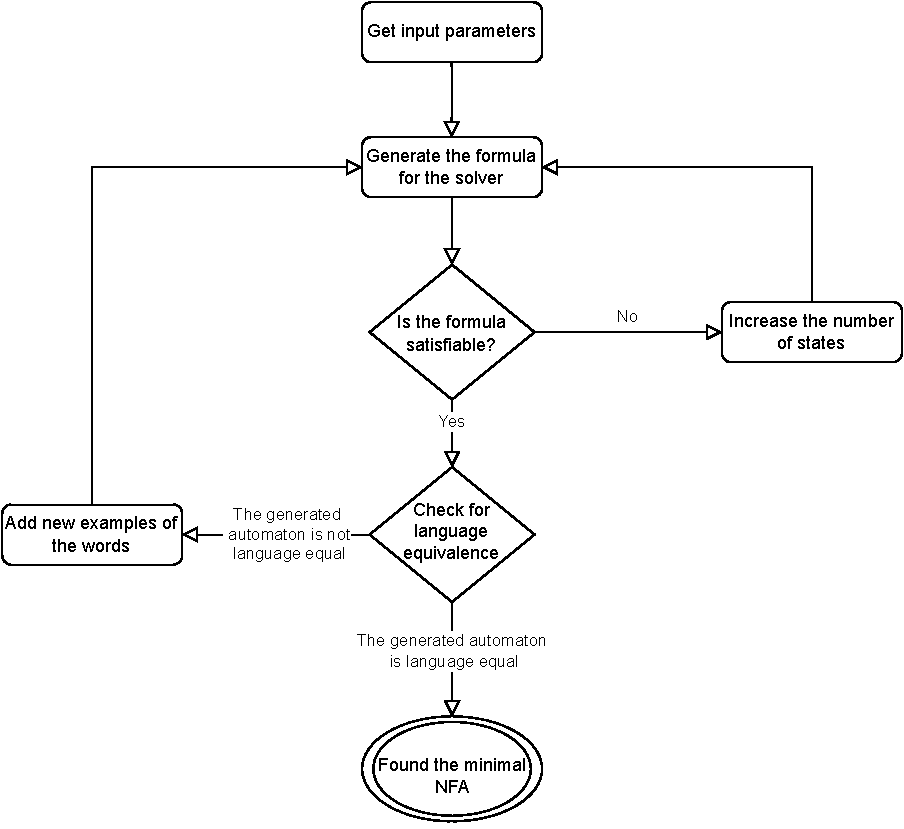
\includegraphics[width=0.8\linewidth]{obrazky-figures/sat_qbf_alg.drawio.pdf}
    \caption{Flowchart of the reduction algorithm using SAT and QBF solvers. The algorithms start by obtaining input parameters which are the number of states and symbols of the automaton, and two sets of example words, one that is accepted and one that is rejected. From there the algorithm runs in a loop updating these parameters until a language-equivalent automaton is found.}
\end{figure}
\vspace{0.3cm}

\chapter{Implementation}
\label{chap:implementation}

For our work, we implemented a program for the reduction of the automata through mentioned known algorithms, for SAT and QBF reduction. We decided to write our program in C++ 20 as we mainly focused on the efficiency of each reduction, meaning that we wanted our implementation to be as fast as possible.

In this chapter, we will explain the finer details of the implementation of our application. Firstly we will talk about the structure of the automaton used for representing the FSAs within the program. Then we specify the file format in which the automata are expected to be for input. For SAT and QBF solvers, we describe the interface for communication between the solvers and our implementation. Lastly, we describe the file formats requested by the solvers and mention the specifications that each solver requires. 

\section{Automaton Structure}
Even though there exist numerous libraries for finite state automata and basic operations over them, we wanted to define our own structure. In this manner, we can design our program to only include components that are required for our application while having the ability to perform any necessary optimizations. 

If we try to follow the formal definition of the automaton, the class \verb|automata| (see Figure \ref{fig:automata_diagram}) representing an FSA would have to define the states of the automaton, its alphabet, transitions, and initial and final states. Since a transition consists of two states and a symbol, it is probably the most challenging aspect to specify. None of these parameters are unique for a transition in an NFA and cannot be used to identify it in the automaton. For this reason, we defined a class \verb|auto_state| to represent the state of the automaton, which can then store all of the transitions leading from this state using pointers (see Figure \ref{fig:state_diagram}). The \verb|automata| class then holds the table with every state in the automaton.

\begin{figure}[ht]
    \label{fig:automata_diagram}
    \centering
    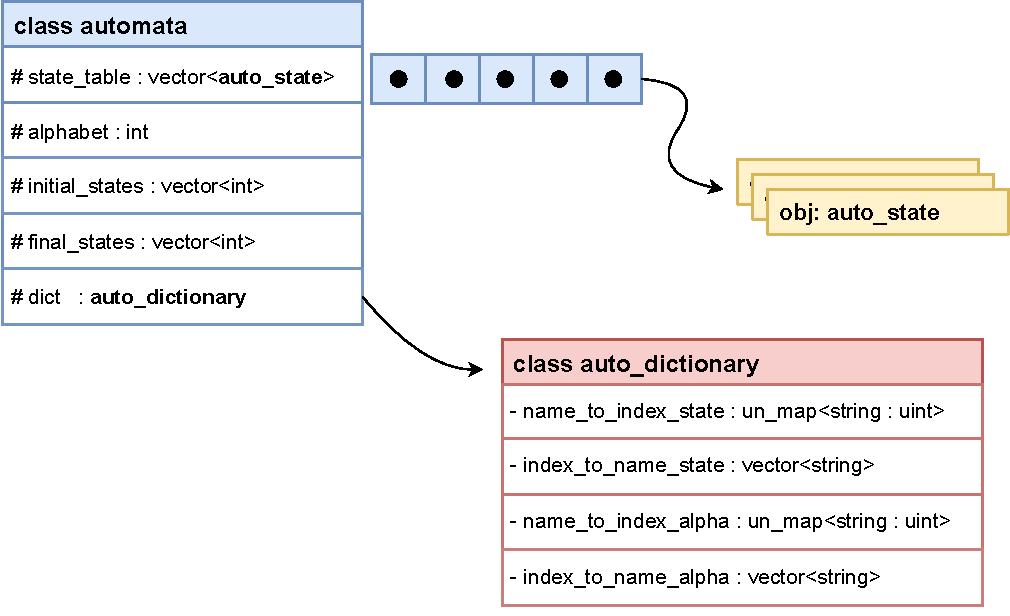
\includegraphics[width=0.9\linewidth]{obrazky-figures/automata_class.pdf}
    \caption{Diagram visualizing the \texttt{automata} and \texttt{auto\_dictionary} classes with their attributes. The blue array represents the vector of pointers to instances of \texttt{auto\_states} indicated by the arrow. The alphabet of the automaton can be described by a single number holding its size. Initial and final states hold values of indices of states with the corresponding property. Class \texttt{auto\_state} is described in Figure \ref{fig:state_diagram}.}
\end{figure}
\vspace{0.3cm}

Typically, the numbers are used to represent the states of the automata and letters for the symbols of the alphabet. As there is no established maximum size for the automaton's alphabet, 26 letters of the English alphabet would not be sufficient. We did not want to limit the input format to integers only, leading to using strings as the data structure holding the value of the alphabet's symbols.

A similar issue arises during the determinization process when a group of states is merged and represented as a single state. The value for the newly created state should somehow reflect the states it was formed from. For this purpose, we utilized the concatenation of string values of the states. However, using strings in a program can be rather costly and time-consuming as they require a lot of work around them.

To provide a better solution, we defined a class \verb|auto_directory| as a directory translating the values of the states and symbols of the alphabet to a unique index. This way, we minimize the amount of additional processing required. \\

\begin{figure}[!hb]
    \label{fig:state_diagram}
    \centering
    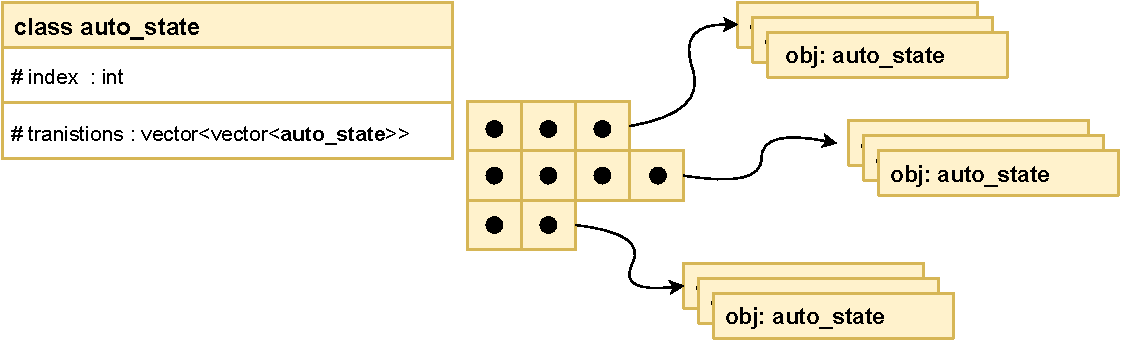
\includegraphics[width=0.9\linewidth]{obrazky-figures/state_class.pdf}
    \caption{Diagram presenting the class \texttt{auto\_state} and its attributes. The class consists of an integer holding the state's index and a 2D vector of pointers to instances of the \texttt{auto\_state} class. Each row can represent a symbol of an alphabet and each pointer in a row a transition leading through the symbol to the referenced state.}
\end{figure}
\vspace{0.3cm}

With the structure defined, we implemented the selected methods of reduction. To ensure that the automaton's languages remained the same after the reduction, we also needed a means to verify its equivalence. The language comparison was implemented through the intersection with the complements as well as through antichains mentioned in Section \ref{sec:dfa}. The reduced automaton can be saved into the output file once it has been confirmed that the reduction was successful.

\section{Automata Files}

The input format of the desired automaton into the application is in the form of a path to a \verb|.vtf| (VATA format) file. The parser will process the given file with the automaton’s structure and create an instance of the \verb|automata| class based on the contents of the file. This format originates from the VATA library \cite{VATA_lib}, which was designed to efficiently manipulate NFAs with an emphasis on utilizing them for static verification. The format describes the syntax for various automata and transducers \cite{VTF_files}. The NFA syntax is sufficient for our purposes and is the only one that the parser will accept. The format of the files consists of single-line definitions of the elements of the automaton, which is described using Backus–Naur form-like grammar in Figure \ref{fig:bnf_grammar}:

\begin{figure}[ht]
\label{fig:bnf_grammar}
\begin{verbatim}
<FILE>                ::= <COMMENT><HEADER><BODY>
<COMMENT>             ::= "@" <TEXT> eol
                        | ""
<HEADER>              ::= <HEADER_LINE><HEADER_LINE><HEADER_LINE>
<HEADER_LINE>         ::= "%"<IDENTIFIER> <TOKEN_LIST> eol
<IDENTIFIER>          ::= "Initial"
                        | "Final"
                        | "States"
<TOKEN_LIST>          ::= <TOKEN> <MORE_TOKEN_LIST>
<MORE_TOKEN_LIST>     ::= <TOKEN> <MORE_TOKEN_LIST>
                        | ""
<BODY>                ::= <TRANSITION> <BODY>
                        | ""
<TRANSITION>          ::= <TOKEN> <TOKEN> <TOKEN> eol
<TEXT>                ::= <PRINTABLE><MORE_TEXT>
<MORE_TEXT>           ::= <PRINTABLE><MORE_TEXT>
                        | " "<MORE_TEXT>
                        | ""
<TOKEN>               ::= <PRINTABLE><MORE_TOKEN>
<MORE_TOKEN>          ::= <PRINTABLE><MORE_TOKEN>
                        | ""
<PRINTABLE>           ::= ASCII printable character
\end{verbatim}
\caption{Syntax of the \texttt{.vtf} file described through Backus–Naur form-like grammar that is expected as input for the creation of the automaton in the program.}
\end{figure}

In Figure \ref{fig:vtf_example} we present an example of a file in \texttt{.vtf} format defining an NFA with five states.

\begin{figure}[!hbt]
\label{fig:vtf_example}
\begin{verbatim}
@ NFA with N=5, S=2
%States q0 q1 q2 q3 q4
%Initial q0
%Final q4

q0 a q2
q0 b q0
q1 a q1
q1 b q2
q2 a q4
q3 a q3
q3 a q4
q4 b q3
\end{verbatim}
\caption{An example of \texttt{.vtf} file used as an input format with the automata structures. Defines an automaton with five states and an alphabet with two symbols. Transitions in the automaton are defined in the body of the file with each transition on a single line in the format: \texttt{from\_state} \texttt{symbol} \texttt{state\_to}}
\end{figure}


\section{Interface for SAT and QBF Solvers}
For the reduction utilizing SAT and QBF solvers, we needed to develop an interface that could communicate between our application and the solver. We implemented a simple bash script that handles the entire communication between different components through files. The script can store the input parameters for the formula generation, which will be updated throughout the process. We tested different SAT and QBF solvers to find the most suitable one for our problem. From SAT solvers we tried \texttt{MiniSat\_v1.14} \cite{MiniSat_page} and  \texttt{Kissat} \cite{Kissat_page} solvers and from QBF solvers it was \texttt{CAQE} \cite{CAQE_page}, \texttt{DepQBF} \cite{DepQBF_page}, and \texttt{Qute} \cite{QUTE_page}.

The result of our program is saved in a file in a format required by the solver (more details in Subsection \ref{sec:input_solvers}). Additionally, the interface assists in unifying the output format of the solver, which varies from solver to solver. In most cases, the output from the solver comes in the form of values that the responding variables should hold for the formula to be satisfiable. Since the order of the variables is essential in our situation, we demand them to be in the ascending order. This output is saved in a file \verb|result.txt| from which it is then retrieved for comparison with the original automaton.

Due to the fact that this algorithm runs in a loop that mostly adds example words, a large number of the clauses are produced redundantly.
A solution could be only adding clauses for the newly discovered words without altering the previously generated formula if its change is not required (for instance, as a result of increasing the number of states). However, only a single solver from the ones we tested gives us this possibility. Most of the time, solvers demand a header with the number of clauses and variables they will be dealing with in advance, especially QBF solvers that also require precisely defined quantified variables. The number of clauses changes every iteration prompting an adjustment to the header. Whenever the number of states increases, all clauses for accepting and rejecting the sets of words must be constructed from the start, as the variables defining the automaton (transition, initial and final variables) change.

Although working with files might be costly in processing time, solvers require an input file as an argument, and their output is not unified as some print their result to the \verb|stdout| while others into the given output file.

\subsection{Notation for Words for CNF Formula Generation}

Since we represented the symbols of the alphabet as indices, we intended to maintain this notation while creating the CNF formula to minimize the usage of strings. For the generation of the formula, the symbols themselves are not as significant as how many of them there are. If the symbols are always described through the same notation, using numbers will not cause any issues. A word is then defined as a collection of numbers. 

These words need to be preserved through multiple iterations of the reduction loop so that they can be then used as command line arguments. Arguments for C++ applications are represented as strings by default, leading us to use the notation for a word as a string of numbers separated by spaces. From this point forward, this notation will also be used throughout the thesis to represent words that an automaton accepts or rejects for CNF formula generation. For instance, the expressions \texttt{``0 1 0''} and \texttt{``1 1''} would be equivalent to the words \textit{``aba''} and \textit{``bb''} with $\Sigma=\{a,b\}$.

\subsection*{Transformation to CNF}
We decided to implement the transformation to CNF through the \textbf{Tseytin transformation} since it gives a linear expansion of the DNF clause. The input clause is a disjunction of subclauses $S_1, S_2,..., S_x$, each being a conjunction of literals. We tried to optimize the transformation to reduce the number of clauses and generated variables by creating a gate per subclause. One additional gate is needed to define the disjunction of these subclauses.

It holds that if $|S_n|$ is the number of literals of the subclause $S_n$ then it can be substituted by $|S_n|+1$ clauses in CNF denoting the same operation. As the output of the final \textit{OR} gate must be set to be \textit{true} for the resolution to work correctly, we can define the \textit{OR} gate by only a single clause saying that at least one of the inputs has to be true.

Let $(A \land \neg B \land C)\lor(\neg D \land  \neg E \land F)$ be the input DNF clause with two subclauses for the Tseytin transformation. The gate representation is shown in Figure \ref{fig:Tsei_opt}.

\begin{figure}[ht]
    \label{fig:Tsei_opt}
    \centering
    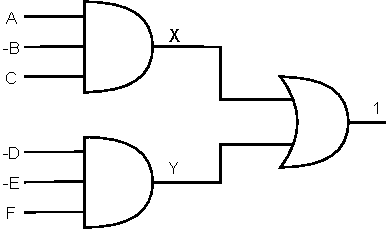
\includegraphics[width=0.5\linewidth]{obrazky-figures/Tseitin_opt.drawio.pdf}
    \caption{Gate representation of the formula $(A \land \neg B \land C)\lor(\neg D \land  \neg E \land F)$ for Tseytin transformation with output of \textit{OR} gate set to \textit{true}.}
\end{figure}

The CNF clause equivalent would then be represented by two sets of clauses for each \textit{AND} gate:

\begin{center}
    \begin{tabular}{c c c c}
      $(A \lor \neg X)$ & $\land $ & $(\neg D \lor \neg Y)$ & $\land $\\
      $(A \lor \neg X)$ & $\land $ & $(\neg E \lor \neg Y)$ & $\land $ \\ 
      $(C \lor \neg X)$    &  $\land $ &  $(F \lor \neg Y)$   & $\land $\\
      $(\neg A \lor B \lor \neg C \lor X)$    & $\land $ &    $(D \lor E \lor \neg F \lor Y )$  &\\
\end{tabular}
\end{center}

And a single clause for the \textit{OR} gate that forces at least one of the inputs to be true.
\begin{align*}
    X \lor Y
\end{align*}


\section{Input Formats for the Solvers}
\label{sec:input_solvers}
SAT and QBF solvers denote their own file formats that are requested as input. These formats are similar as both of them include a formula in CNF. The main distinction is the header. Some specific solvers require even more specifications added for them to be able to operate on the provided file. In this section, we will discuss the \texttt{DIMACS} file format needed by SAT solvers and the \texttt{QDIMACS} format required by QBF solvers, and how each employed solver for the testing needs its input defined.

\subsection{CNF File Format}
The most common input file type for SAT solvers is the \verb|DIMACS| format \cite{DIMACS_page}. This format is fairly straightforward as it only has three components: optional comment lines, a header with a single problem line, and a body containing the CNF formula.
\begin{itemize}
    \item The \textbf{comment line} is marked with a letter \emph{c} in the beginning indicating that the solver will ignore everything up until the end of the line.
    \item The \textbf{problem line} has the syntax: \texttt{p cnf X Y}, where \emph{X} is the number of variables, and \emph{Y} is the number of clauses in the following formula. 
    \item The \textbf{body} consists of CNF clauses, each written on a single line with the symbol \emph{0} designating the end of the phrase and the logical operator \textit{AND}. The clause is defined as a set of numbers separated by spaces, where numbers represent the variables and space represents the logical operator \textit{OR}. Negative numbers are assigned to the respective variables in the clause to symbolize their negation.
\end{itemize}

\begin{figure}[ht]
\label{fig:cnf_example}
\begin{verbatim}
c example_cnf_file.cnf
c Automaton with N=2, S=1, Acc={"0"}, Rec={"0 0"}
c
p cnf 8 15
-1 -2 0
-3 -4 0
1 2 0
3 4 0
1 -7 0
5 -7 0
-1 -5 7 0
2 -8 0
6 -8 0
-2 -6 8 0
7 8 0
-1 -1 -5 0
-1 -2 -6 0
-2 -3 -5 0
-2 -4 -6 0
\end{verbatim}
\caption{Syntax of the \texttt{.cnf} file in DIMACS format requested by the majority of SAT solvers. The file starts with comment lines, followed by the problem line, and, finally, the body with the formula in CNF.}
\end{figure}

In Figure \ref{fig:cnf_example} we show an example of a \verb|.cnf| file that would be created for finding an automaton with $N=2$, $|\Sigma|=1$, accepting the word \texttt{``0''}, and rejecting the word \texttt{``0 0''}.

In our work, from the SAT solvers, we tested the \texttt{MiniSat} and the \texttt{Kissat} solvers. The input format for \texttt{Kissat} is a standard \verb|.cnf| file. The problem line is not necessary for \texttt{MiniSat} to be able to solve the given formula, though. As the absence of the header does not have a noticeable effect on the solver's performance, we can exploit this property by adding new clauses without the need to modify the header. As a result, a substantial part of the formula in the file would not need to be produced from the start.

\pagebreak
\subsection{QDIMACS File Format}
On the other hand, QBF solvers require input files in \verb|QDIMACS| format \cite{QDIMACS_page}. This format is similar to the \verb|DIMACS| one since both have the same syntax for comment lines and the body with the CNF formula. The only difference is the header, which, besides the problem line, also requires defining which variables are existential and which are universal. That is accomplished by adding \textbf{quantifying lines} after the problem line. These lines begin with the letter \emph{e} for marking the existential variables and \emph{a} for universal variables. Those are then followed by a group of positive numbers representing variables that belong to the particular quantifier, and the line is then ended with the symbol  \emph{0}. The same quantifier cannot appear in two consecutive lines, one right after another. In general, an existential quantifier is assigned to every non-quantified variable. 

\begin{figure}[ht]
\label{fig:qdimacs_example}
\begin{verbatim}
c example_qdimacs_file.qdimacs
c Automaton with N=2, S=2, Acc={"0 1"}
c
p cnf 15 13
e 13 14 15 0
9 0
13 9 0
-13 10 0
15 11 0
-15 12 0
13 14 1 0
13 -14 2 0
-13 14 3 0
-13 -14 4 0
14 15 5 0
14 -15 6 0
-14 15 7 0
-14 -15 8 0
\end{verbatim}
\caption{Syntax of the \texttt{.qdimacs} file required by QBF solvers, containing a quantifying line with the existential variables.}
\end{figure}

In Figure \ref{fig:qdimacs_example} we present a \verb|.qdimacs| file holding the formula for the automaton with $N=2$, $|\Sigma|=2$, and accepting the word \texttt{``0 1''}.

We put to the test three QBF solvers, which are \texttt{CAQE}, \texttt{DepQBF}, and \texttt{Qute}. Only \texttt{Qute} has the unique requirement that every variable needs to be quantified. Since this solver does not support non-quantifiable variables, we must assign an existential quantifier to each non-quantifiable variable, which would be the variable assigned automatically.

\chapter{Experimental Evaluation}
\label{chap:evaluation}

In this chapter, we will discuss the experimental evaluation of the implemented techniques. Our two primary evaluation criteria were the size of the automaton (number of states) and the time required to complete the reduction. Firstly we will compare the results of the reduction algorithms from Chapter \ref{chap:reduction}. Then, we discuss the potential for our reduction algorithm from Chapter \ref{chap:sat_qbf}. Lastly, we present results of reduction utilizing SAT and QBF solver on the selected set of automata. All of the tests were carried out on a laptop, an \texttt{Intel(R) Core(TM) i5-8300H CPU} at \texttt{2.30GHz} with \texttt{8.00GB} of RAM. Source files were compiled using \texttt{g++} with optimization option \texttt{-O2} for better execution time.

\section{Effectiveness of Selected Reduction Algorithms}

The reduction algorithms, specifically the minimization of DFA through Hopcroft's and Brzozowski's algorithm, the reduction based on a relation of simulation, and the reduction by transformation into a CRSA, were run on a selection of 4\ 042 automata from regular model-checking \cite{armcNFA_page} with sizes up to almost 4\ 000 states and various alphabets. These reductions were implemented following the algorithms in Chapter \ref{chap:reduction} without any extra optimization; the reduction based on the simulation relation was consisting of creating this relation for the input automaton and utilizing its symmetric fragment to find sets of states that can be represented as one.

The reduction algorithms were run sequentially on the same automaton, and the success of each reduction was confirmed by a language inclusion checking using antichains. The time for the reduction was measured using the \texttt{clock()} function in C++ library \texttt{<ctime>} as the difference of time before and after the reduction. In Figure \ref{fig:graph_eff} are the results of the effectiveness of the performed reduction shown as the comparison of the size of the original and reduced automaton. In Figure \ref{fig:graph_time} is presented a graph of time that was required for every type of reduction based on the size of the input automaton.

\begin{figure}[ht]
    \label{fig:graph_eff}
    \centering
    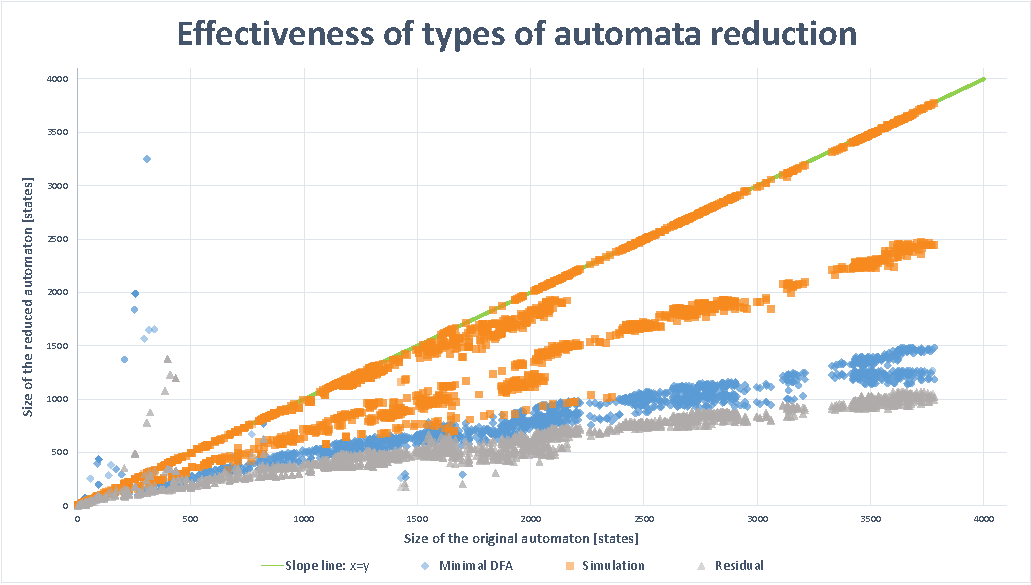
\includegraphics[width=1\linewidth]{obrazky-figures/effectiveness.pdf}
    \caption{Graph presenting the relationship between the size of the original and reduced automaton as the effectiveness of selected reduction algorithms.}
\end{figure}
\vspace{0.3cm}

We can evaluate that minimal DFA and residual automata, with reduction utilizing RSAs having the best results for the chosen set, often outperforming reduction through the relation of simulation.

We can observe three slope lines for the reduction through simulation, with the slope line \texttt{x=y} being one of the most frequently followed, indicating that no states that would be simulated and could be merged, were found. From our example set, there were 521 instances for reduction using simulation where the size of the provided automaton underwent absolutely no reduction at all. The effectiveness of this reduction type strongly depends on the simulation relation found on the given automaton. Overall, the average reduction in the size of the automaton obtained through simulation is just 16.47\%, including both the successful and unsuccessful reductions. On the other hand, in the worst situation, this type of reduction results in an automaton that is of the same size as the original one.

For the reduction using minimal DFAs or RSAs, there exists a possibility that the automaton will grow in size instead of reducing it. A few examples of 400-state automata growing into a few thousand-state ones can be seen in the graph. It is the result of utilizing determinization in both algorithms. In our selection, 253 minimal DFAs actually grew in their size after reduction. As the provided automaton may be an NFA, this phenomenon is not uncommon, and the state number increase after the determinization is anticipated. However, the minimal DFA reduction was 42.36\% on average, significantly outperforming the reduction through simulation.

The reduction using residual automata had only 42 occurrences when the result automaton was larger than the original one, leading to the average reduction being 61.20\%, which means that the reduced automaton was typically smaller than half of the size of the original one. For our selected automata, we can state that most of the time, the reduction through minimal DFA and transformation into CRSA offers sustainably exceptional outcomes.



\begin{figure}[ht]
    \label{fig:graph_time}
    \centering
    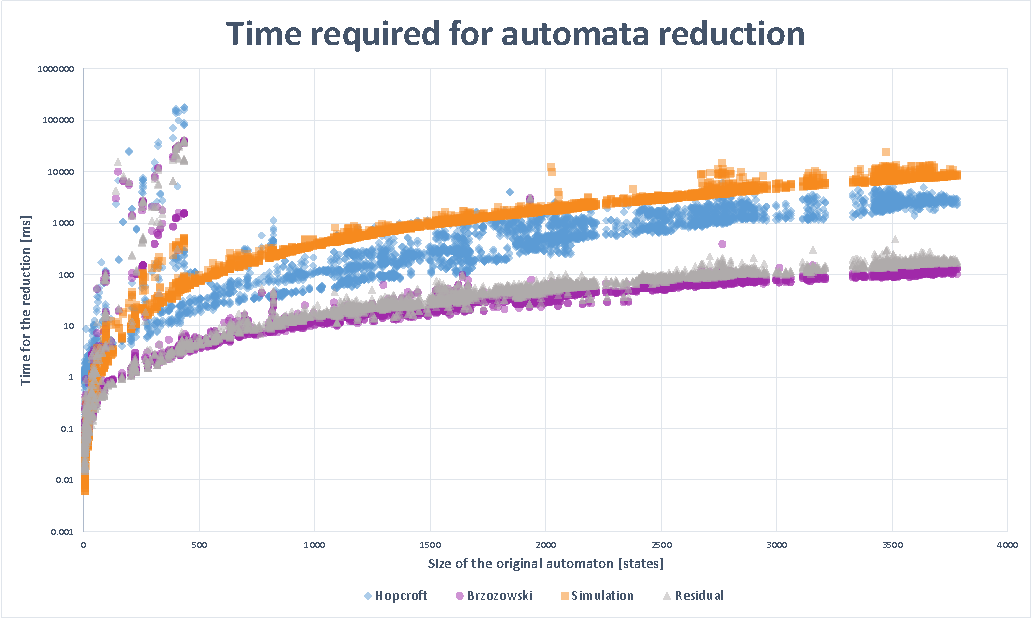
\includegraphics[width=1\linewidth]{obrazky-figures/time.pdf}
    \caption{Graph visualizing the time required to run each type of reduction based on the size of the original automaton.}
\end{figure}
\vspace{0.3cm}

The time results in Figure \ref{fig:graph_time} provide similar outcomes based on the type of the reduction, with reduction using residual automata and Brzozowski's algorithm for minimal DFA producing the best results, followed by Hopcroft's algorithm, and the simulation coming in last. The reduction by transformation into CRSA and Brzozowski follow the same pattern due to both requiring double determinization, with CRSA also containing the removal of coverable states, which takes some additional time. Same as in the previous graph, we can find quite a few cases of irregularities for every algorithm requiring determinization for the automata up to the size of 500 states.

Firstly, these fluctuations result from the occurrences of automata for which minimal DFA was incomparably larger than the initial NFA. Since Hopcroft's and Brzozowski's algorithms had to deal with thousands of states of the final automaton, those reductions took longer to complete. Regarding the residual reduction, even though in these cases the final automaton was approximately two times larger than the initial one, the reduction time did not add up when compared to the other outcomes of this reduction for much larger automata.

After closer inspection, we found that the additional time needed for reduction utilizing CRSAs is merely due to the requirement for backward determinization. The coverable states are eliminated during the reduction process, so they do not appear in the final automata, but the determinization can still lead to exponential growth, just like for the minimal DFA. In this manner, the reduction may pointlessly produce thousands of states only to remove them afterward, taking extra time.

In our situation, the results for Brzozowski and CRSA may be favorable, which is primarily caused by the backward determinization being the correct choice, typically providing reduction rather than expansion of the given automata. For some automata, however, this might not be the case because the determinization could result in exponential growth, which is the weakness of these reductions. There are no such drawbacks for the reduction through the relation of simulation in terms of time, but it is clear that it generally takes longer than the other reductions. The average time of our implementation for these reductions is around the one-second mark when approaching 4\ 000 state automata.

\subsection{Comparison against different implementations}

Comparison of the effectiveness of our implemented algorithms against the results of different approaches may be difficult as there may be a lot of imprecise details, such as the machine used for the tests, the sample set of automata, the programming language used, the constructions, optimization used on the given algorithm and more. There exist studies that performed similar experiments on the effectiveness of reduction algorithms for FSAs and implemented Hopcroft's and Brzozowski's algorithms. 

The article \textit{On the performance of automata minimization algorithms} \cite{Almeida2007} used the programming language Python while experimenting with automata up to the size of 100 states with various alphabets. However, after 24 hours, their algorithms would time out for their random deterministic automata with 100 states and alphabets of size 10. The thesis \textit{The Practical Performance of Automata Minimization Algorithms} \cite{Veen2017} provides better results in C++ outperforming even our implementation when it comes to the time required for the reduction. Their Hoproft's algorithm features some optimizations that were not included in our version, and the tests were run on a more powerful machine. Still, our results are not far behind and could be comparable if evaluated under the same conditions.

\section{Possibilities of Utilizing SAT and QBF Solvers for Reduction}

Our reduction algorithm utilizing SAT and QBF solvers presented in Section \ref{sec:sat_qbf_alg} is dependent on various factors such as the number of iterations of the reduction required to find an equivalent automaton, words defining the automaton's language, the number of symbols of the alphabet, and the number of states. We wanted to present a way to evaluate the possibilities of the given algorithm in general, so we took the number of clauses as a potential main evaluation criterion as it directly correlates with the input parameters representing the automaton as well as with the solver.

\begin{figure}[hbt]
    \label{fig:graph_clauses_SAT_QBF}
    \centering
    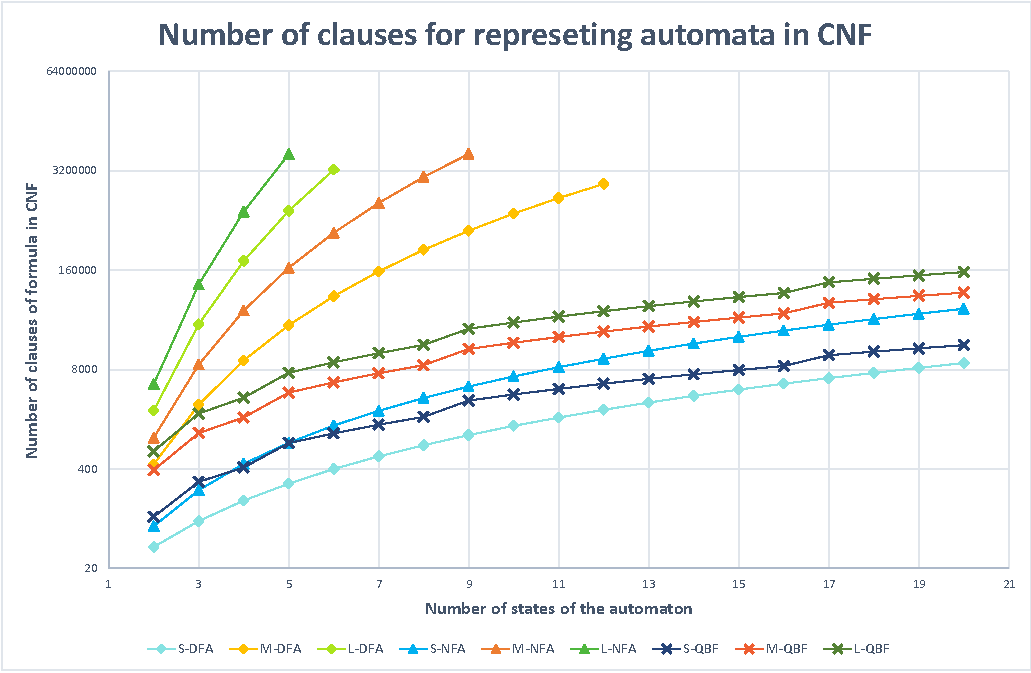
\includegraphics[width=1\linewidth]{obrazky-figures/clauses_for_SAT_QBF.pdf}
    \caption{Graph presenting the number of clauses generated for the automata representation in Boolean algebra based on its number of states. The symbols of the alphabet were set to the constant number of two. Each type of representation: DFA~(SAT), NFA~(SAT), and QBF was tested on three types of input word sets, each with a different size: \linebreak {S -- max $l = 2$}, {M -- max $l = 5$}, {L -- max $l = 7$}, where $l$ is the length of the input word.}
\end{figure}

Figure \ref{fig:graph_clauses_SAT_QBF} shows a graph visualizing the number of clauses required to represent the selected automaton based on its number of states, where $|\Sigma|=2$ and $ 2 \leq N \leq 20$. Three different types of input word sets, ranging in size from small -- S (2 words per set) to big -- L (7 words per set), were constructed for each representation (DFA -- SAT, \linebreak NFA -- SAT, and NFA -- QBF). The timeout for both generation and solving was set to 15 minutes.

For SAT solvers, we may observe an exponential increase in the number of clauses based on the given input. As mentioned in Chapter \ref{chap:sat_qbf}, the number of clauses necessary to represent the acceptance or rejection of the words by the automaton can be expressed as $N^l$ for DFA and $N^{l+1}$ for NFA with $l$ being the length of the word. Since the clauses for accepting the word are in DNF and must be converted into CNF, the number increases even further. This amount of clauses becomes unbearable for larger automata when we get millions of clauses for the large input set after reaching just five states. For this reason, we included QBF solvers for our algorithm, allowing us to reduce the number of clauses from exponential growth to quadratic, represented by the expression ${l \times N^2}$, thanks to the quantified variables. For 20-state automata with the large input word set, we still only get around 150\ 000 clauses.

\vspace{0.3cm}

As the reduction algorithm depends not only on the algorithm itself but also on the solver, we experimented with a few different solvers to identify the most suitable one for our needs. Figure \ref{fig:graph_SAT_compare} presents results of testing the performance of \texttt{MiniSat} and \texttt{Kissat} solvers as the time required to solve the given formula by the solver.

\begin{figure}[ht]
    \label{fig:graph_SAT_compare}
    \centering
    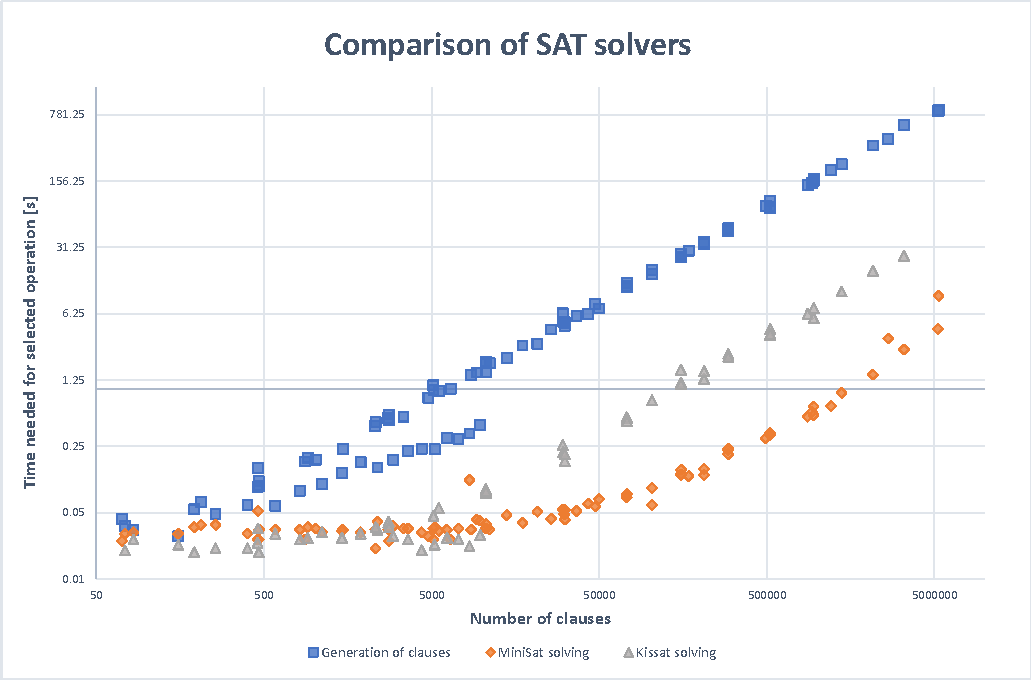
\includegraphics[width=1\linewidth]{obrazky-figures/SAT_comparison.pdf}
    \caption{Graph illustrating the time required to solve the given formula by \texttt{MiniSat} and \texttt{Kissat} solvers based on the number of clauses of the formula. For comparison is also shown time needed for generating the formula. Both axes of the graph are logarithmic.}
\end{figure}
\vspace{0.3cm}

Both solvers perform almost alike up to around 5\ 000 clauses with only a few tens of milliseconds needed. From there, the better scaling solver is \texttt{MiniSat} running five times faster on larger formulas than \texttt{Kissat}. However, both solvers deliver excellent results in a matter of seconds, even when dealing with hundreds of thousands of clauses. This time is essentially insignificant compared to the time required for the generation of the formula into the file. The more suitable solver chosen for our reduction is \texttt{MiniSat} not only for its slightly better performance but mainly because of its property that allows it to solve the given formula without requiring any header with additional details about the formula at all as was described in Chapter \ref{chap:implementation}. 

Similar experiments were carried out on selected QBF solvers. In contrast to SAT solvers, the performance of QBF solvers is not implied by any function or rule. Furthermore, it appears that each solver has a maximum number of clauses that it can handle and that once this limit is exceeded, the solver's processing time increases exponentially. The solving time does not depend only on the number of clauses or variables but also on the structure of the clauses meaning that the solver may need just a few milliseconds or several seconds to solve the same number of clauses. We present selected results in Table \ref{tab:QBF_compare} to give an overview of the general performance of each solver.

\begin{table}[hb]
    \centering
    \label{tab:QBF_compare}
    \caption{Comparison of performance of selected QBF solvers for the given clauses. Added also the time required for the generation of clauses for comparison. The timeout was set to 10 minutes.}
    \vspace{0.3cm}
    \begin{tabular}{|c||c|c|c|c|c|c|c|} \hline
        \textbf{Number of clauses} & 535 & 1\ 168 & 1\ 922 & 2\ 448 & 3\ 137 & 5\ 210 & 8\ 898 \\ \hline \hline
        \textbf{Generation time} & 0.11s & 0.30s & 0.42s & 0.52s & 0.67s & 1.07s & 1.92s \\ \hline
        \textbf{CAQE time} & 0.08s & 0.13s & 0.18s & 0.23s & 0.69s & 1.12s & 2.24s \\ \hline
        \textbf{DepQBF time} & 0.03s & 0.17s & 0.99s & 0.13s & 3.37s & 6.18s & 311.57s \\ \hline
        \textbf{Qute time} & 0.12s & 2.50s & 5.03s & 0.58s & 201.35s & - & - \\ \hline
    \end{tabular}
\end{table}

\texttt{Qute} started showing difficulties when given roughly 4\ 000 clauses and started getting timed out. \texttt{DepQBF} was performing well up to 9\ 000 clauses. The most reliable results offered \texttt{CAQE}, which can still handle 10,000 clauses but takes around 30 seconds to solve the formula. It is the exact opposite when compared to SAT solvers. In this instance, the time required for the solver is significantly longer than the time necessary for formula generation. Even though we can express an automaton for QBF solvers in considerably fewer states than for SAT solvers, the QBF solvers require longer execution times, even for the smaller formulas.


\section{Results of SAT and QBF-based Reduction}

With solvers selected and assumptions about the real possibilities of this reduction algorithm, we created a collection of benchmark automata with increasing complexity. The previous tests have demonstrated that the amount of clauses will be crucial for the usability of the reduction. Two main factors affecting the number of clauses are the number of states of the automaton and the sets of sample words. 

For the automaton size, we focused our benchmark set on small automata starting from only three states, from which they will progressively grow in size. Since we would be working with smaller automata, we set the automaton's initial size to be equal to half of the original size and then gradually increase it. The characterization of the automata in the benchmark set can be seen in Table \ref{tab:benchamrks} noting the number of states ($N$), number of symbols of the alphabet ($|\Sigma|$), and the language that the automaton defines.

In order to minimize the number of clauses for the sample words, we concentrated first on finding the shortest words defining the automaton's language. For this reason, the breadth-first search was used when traversing the automaton. Firstly we search for words with maximum lengths no greater than the automaton's shortest accepted word (except for epsilon). When comparing the languages of the automata, we take similar precautions by limiting the length of the found words to just the first shortest ones found and setting the maximum number of counterexamples to three. Even though we may end up with more iterations to discover enough words to define the language, it will ensure that the words are introduced in small patches. Otherwise, even a three-state automaton could find a word with a length of 8, which would needlessly prolong the generation and solving time for numerous clauses.

\begin{table}[hb]
    \centering
    \label{tab:benchamrks}
    \caption{Characterization of the benchmark set of automata used for reduction using SAT and QBF solvers. Contains a number of states, symbols of the automaton, and its language.}
    \vspace{0.3cm}
    \begin{tabular}{|c||c|c|c|} \hline
        \textbf{Benchmark} & $\boldsymbol{N}$ & $\boldsymbol{|\Sigma|}$ & \textbf{Language} \\ \hline \hline
        \textbf{A} & 3  & 1 &  $aa$ \\ \hline
        \textbf{B} & 3  & 2 &  $b^*a(b|(aa))^*$\\ \hline
        \textbf{C} & 4  & 2 &  $aaa(a|b)^*$ \\ \hline
        \textbf{D} & 4  & 2 &  $(baa^*a)^*(ba|(a)a^*$\\ \hline
        \textbf{E} & 4  & 3 &   $(cc^*aa^*bb^*)|(aa^*bb^*)|(bb^*)(cc^*aa^*bb^*)^*$\\ \hline
        \textbf{F} & 4  & 7 &  $(a|b)(a|b)(a|b)(a|b|c|d|e|f|g)^*$  \\ \hline
        
    \end{tabular}
\end{table}

We tested every representation, DFA for SAT, NFA for SAT, and NFA for QBF, on the same benchmark set. Throughout the run of the benchmarks, we noted characteristics defining the reduction run, including the number of states of the reduced automaton ($N'$), the number of iterations on the reduction cycle, the number of words defining the automaton's language (accepting and rejecting words), the number of clauses of the final formula, the sum of times required for the generation of clauses, and the total time needed by the solver. In Table \ref{tab:dfa_minisat_results} are summarised results for the DFA and NFA reduction, both using SAT solver \texttt{MiniSat}, together with the results for NFA reduction utilizing the QBF solver \texttt{CAQE}.

\begin{table}[ht]
    \centering
    \label{tab:dfa_minisat_results}
    \caption{The summary of results of testing the reduction utilizing SAT solver \texttt{MiniSat} for finding a minimal DFA and NFA, and results of the reduction utilizing QBF solver \texttt{CAQE} for NFA reduction.}
    \vspace{0.3cm}
    \begin{tabular}{|c||c|c|c|c|c|c|c|} \hline
         \multirow{2}{*}{\textbf{Benchmark}} & \multirow{2}{*}{$\boldsymbol{N'}$} & \multirow{2}{*}{\textbf{Iterations}} & \multicolumn{2}{c|}{\textbf{Words}} & \multirow{2}{*}{\textbf{Clauses}} & \textbf{Generation} & \multirow{2}{*}{\textbf{Solve time}}\\ \cline{4-5}
            &       &       &    Acc    &   Rej     &       &   \textbf{time}   &\\ \hline \hline
           \multicolumn{8}{| c |}{\textbf{DFA -- SAT}} \\ \hline
        \textbf{A} &  4  &    6     &   1    &     5     &   5\ 474  & 0.203s   &   0.193s \\ \hline
        \textbf{B} &  4  &    16     &   5    &     12     &   20\ 302  & 0.964s   &   0.615s \\ \hline
        \textbf{C} &  5  &    18     &   3    &     19     &   38\ 849  & 2.937s   &   0.718s \\ \hline
        \textbf{D} &  6  &    20     &   5    &     15     &   72\ 510  & 16.354s   &   1.067s \\ \hline
        \textbf{E} &  5  &    32     &   7    &     27     &   107\ 448  & 3.887s   &   1.382s \\ \hline
        \textbf{F} &  5  &    61     &   15    &     95     &   172\ 361  & 9.759s   &  3.221s \\ \hline \hline
        \multicolumn{8}{| c |}{\textbf{NFA -- SAT}} \\ \hline
        \textbf{A} &  3  &    2     &   1    &     2     &   150  & 0.069s   &   0.054s \\ \hline
        \textbf{B} &  3  &    8    &   5    &     4     &  1\ 569  & 0.469s   &   0.225s \\ \hline
        \textbf{C} &  4  &    5     &   3    &     6     &   16\ 299  & 3.442s   &   0.165s \\ \hline
        \textbf{D} &  4  &    11     &   5    &     7     &   187\ 613  & 36.813s   &   0.640s \\ \hline
        \textbf{E} &  3  &    12     &   6    &     8     &   3\ 526  & 0.908s   &   0.340s \\ \hline
        \textbf{F} &  4  &    27     &   25    &     52     &   272\ 039  & 60.036s   &  3.9341s \\ \hline \hline
        \multicolumn{8}{| c |}{\textbf{NFA -- QBF}} \\ \hline
        \textbf{A} &  3  &    5     &   1    &     5     &   882  & 0.476s   &   1.272s \\ \hline
        \textbf{B} &  3  &    7    &   4    &     4     &  593  & 0.357s   &   0.253s \\ \hline
        \textbf{C} &  4  &    8     &   2    &     10     &   2\ 540  & 2.544s   &   1.719s \\ \hline
        \textbf{D} &  4  &    11     &   4    &     8     &   2\ 922  & 2.568s   &   3809.895s \\ \hline
        \textbf{E} &  3  &    15     &   6    &     11     &   2\ 070  & 3.121s   &   1.705s \\ \hline
        \textbf{F}&  4  &    31     &   15    &     73    &   23\ 811  & 100.064s   &  259.683s \\ \hline
    \end{tabular}
\end{table}

For the SAT solver, we can observe that the DFA has overall better results by a small margin as it requires fewer clauses than the NFA with the same number of words. On the other hand, the NFA reduction requires significantly less iterations and uses fewer words to define the automaton's language. For this reason, this method is able to keep up with the deterministic variant. It is important to keep in mind that although the time for creating clauses and solving are the two primary processes in the reduction, the overall run takes much longer due to the additional work involved such as reading and writing files and switching from application to solver. The benchmark F could run for about 30 minutes, despite the fact that the generating and solving time only takes a few minutes. This additional processing time grows even more with a larger number of clauses written in the file

We will notice that the solver is struggling with the QBF representation, and even with only 2\ 000 clauses, the solving of the clauses may take unreasonably long. It demonstrates that the solver's performance is not only determined just by the quantity of clauses. If the clauses do not fit the solver, it could have trouble solving even the smaller formulas. We expected a higher number of iterations because of the limitations to prevent the discovery of needlessly long words. For \texttt{MiniSat} solver, this works well as the new clauses can simply be appended to the end of the file. However, the QBF solver must always create the whole formula from the beginning. Another difference is that QBF solvers take far longer to solve the problems than SAT solvers do for the same input, and excessively running the solver for every new word discovered is not suitable. We attempted to slightly modify the finding of the initial words of the automaton for this reason and looked for words with lengths up to the number of states in the automaton. We ran all three of the representations once more to provide a comparison of a different heuristic for finding the sample words. The results are shown in Table \ref{tab:dfa_minisat_results_2} for every representation. 

\begin{table}[ht]
    \centering
    \label{tab:dfa_minisat_results_2}
    \caption{The results of testing the reduction utilizing SAT solver \texttt{MiniSat} for finding a minimal DFA and NFA, and QBF solver \texttt{CAQE} for NFA with larger initial sample word sets.}
    \vspace{0.3cm}
    \begin{tabular}{|c||c|c|c|c|c|c|c|} \hline
          \multirow{2}{*}{\textbf{Benchmark}} & \multirow{2}{*}{\textbf{$N'$}} & \multirow{2}{*}{\textbf{Iterations}} & \multicolumn{2}{c|}{\textbf{Words}} & \multirow{2}{*}{\textbf{Clauses}} & \textbf{Generation} & \multirow{2}{*}{\textbf{Solve time}}\\ \cline{4-5}
            &       &       &    Acc    &   Rej     &       &   \textbf{time}   &\\ \hline \hline
           \multicolumn{8}{| c |}{\textbf{DFA -- SAT}} \\ \hline
        \textbf{A} &  4  &    6     &   1    &     5     &   5\ 538  & 0.507s   &   0.194s \\ \hline
        \textbf{B} &  4  &    7     &   7    &     12     &   4\ 336  & 0.771s   &   0.206s \\ \hline
        \textbf{C} &  5  &    10     &   3    &     12     &   31\ 174  & 4.028s   &   0.400s \\ \hline
        \textbf{D} &  6  &    14     &   8    &     17     &   136\ 017  & 37.791s   &   1.123s \\ \hline
        \textbf{E} &  5  &    12     &   15    &     60     &   64\ 331  & 11.657s   &   0.557s \\ \hline
        \textbf{F} &  5  &    30     &   64    &     68     &   297\ 085  & 73.138s   &  8.887s \\ \hline \hline
        \multicolumn{8}{| c |}{\textbf{NFA -- SAT}} \\ \hline
        \textbf{A} &  3  &    2     &   1    &     3     &   231  & 0.066s   &   0.061s \\ \hline
        \textbf{B} &  3  &    3    &   7    &     9     &  2\ 892  & 0.617s   &   0.087s \\ \hline
        \textbf{C} &  4  &    3     &   3    &     6     &   16\ 297  & 4.338s   &   0.105s \\ \hline
        \textbf{D} &  4  &    9     &   9    &     12     &   203\ 616  & 39.921s   &   0.516s \\ \hline
        \textbf{E} &  3  &    5     &   15    &     55     &   24\ 593  & 3.630s   &   0.214s \\ \hline
        \textbf{F} &  4  &    11     &   67    &     47     &   520\ 833  & 121.923s   &  5.520s \\ \hline \hline
        \multicolumn{8}{| c |}{\textbf{NFA -- QBF}} \\ \hline
        \textbf{A} &  3  &    4     &   1    &     5     &   882  & 0.517s   &  1.294s \\ \hline
        \textbf{B} &  3  &    4    &   7    &     12     &  2\ 524  & 1.129s   &   2.719s \\ \hline
        \textbf{C} &  4  &    5     &   3    &     8     &   2\ 066  & 1.392s   &   0.551s \\ \hline
        \textbf{D} &  4  &    8     &   8    &     12     &   4\ 174  & 3.697s   &   432.254s \\ \hline
        \textbf{E} &  3  &    7     &   15    &     57     &   12\ 881  & 16.436s   &   34.758s \\ \hline
        \textbf{F} &  4  &    18     &   64    &     58    &   21\ 628  & 88.891s   &  11.922s \\ \hline
    \end{tabular}
\end{table}

Unsurprisingly, even with less iterations of the reduction loop for the SAT solver, we generate more clauses that take longer to create and solve. The longer words that were discovered when initializing the sets of sample words are the primary cause of this. However, the QBF solver performs better despite the number of clauses. As the generation and solving are conducted less frequently, the overall time for reduction decreases. The comparison against results from the previous testing shows the impact of the selected words on the reduction as a whole. These selected optimizations showed the best results, but a more accurate statistic could improve the algorithm's efficiency.


\chapter{Conclusion}
\label{chap:conclu}

The goal of this thesis was to create an efficient implementation of different types of automata reduction to compare their effectiveness on the sample set of automata and propose a new approach to the problem of NFA minimization.

We selected three promising types of reduction that were implemented in C++ and optimized for speed: the minimization of deterministic automata (through Hopcroft's and Brzozowski's algorithms), the reduction based on a relation of simulation, and the reduction by transformation into a canonical residual automaton. We defined our own structure of finite state automaton specifically for these reductions to achieve the best performance. For a collection of 4\ 042 NFAs used for experimental evaluation, the best results were obtained by reductions utilizing backward determination. The average decrease in size for residual automata was 61.20\% from the original size, and the average time needed for the reduction was up to one second. Even if there are undoubtedly possibilities for optimization, our implementation did not fall far behind other implementations with similar algorithms.

We proposed a method of representing a DFA and an NFA as a Boolean formula in CNF that SAT and QBF solvers can use to determine its minimal equivalent. The reduction algorithm involves creating an automaton from sets of example words that will be updated until a language-equivalent automaton is produced. As the automaton's language may be infinite, this reduction primarily focused on proving that such a type of reduction was possible. The testing on a simple set of benchmark automata demonstrated the general possibilities for this algorithm. Although the minimal DFA, as well as minimal NFA, can be found utilizing SAT solvers, using this reduction on general automata is impossible due to the exponentially high number of clauses representing the automaton. As this property was expected, we expanded the method onto QBF solvers, which require only a quadratic number of clauses. However, when compared to SAT solvers, the performance of QBF solvers fell short of expectations.

This thesis offers a solid foundation for further research. For future work, a broader comparison of the residual reduction against the optimized version of Hopcroft's algorithm could give us even more information about the overall performance of this algorithm. For the reduction using SAT and QBF solvers, we have demonstrated how crucial the selection of the words defining the automaton's language is, and additional research in this area could be beneficial for further improvements. Preprocessors and various optimizing tools for QBF solvers can be another alternative method of optimization since the amount of clauses we were working with should be able to be handled without major issues.

%=========================================================================

% For compilation piecewise (see projekt.tex), it is necessary to uncomment it
% \end{document}